\documentclass[
    table,
    12pt,
    oneside,
    a4paper,
    italian
]{book}

\PassOptionsToPackage{dvipsnames}{xcolor} % colori PDF/A

\usepackage{colorprofiles}
% PDF/A
% validate in https://www.pdf-online.com/osa/validate.aspx
\usepackage[a-1a,mathxmp]{pdfx}[2018/12/22]
\usepackage[T1]{fontenc}
\usepackage[utf8]{inputenc}
\usepackage[italian]{babel}
\usepackage{bookmark}
\usepackage{caption}
\usepackage{comment}
\usepackage{chngpage, calc} % centra il frontespizio
\usepackage{emptypage} % pagine vuote senza testatina e piede di pagina
\usepackage{epigraph} % per epigrafi
\usepackage{indentfirst} % rientra il primo paragrafo di ogni sezione
\usepackage{graphicx} % immagini
\usepackage[pdfa]{hyperref} % collegamenti ipertestuali
\usepackage{mparhack,relsize}  % finezze tipografiche
\usepackage{nameref} % visualizza nome dei riferimenti
\usepackage[font=small]{quoting} % citazioni
\usepackage{subfig} % sottofigure, sottotabelle
\usepackage[italian]{varioref} % riferimenti completi della pagina
\usepackage{longtable} % tabelle su più pagine
\usepackage[toc, acronym, automake]{glossaries}
\usepackage[backend=biber, style=verbose-ibid, hyperref, backref]{biblatex}
\usepackage{lmodern}
\usepackage[top=2.75cm, bottom=2.75cm, right=3cm, left=3.75cm]{geometry} % 1in+17pt+0.6cm
\usepackage{fancyhdr}
\usepackage{lipsum}
\usepackage{setspace}
\usepackage{titlesec}
\usepackage[cachedir=minted-caches]{minted} % https://it.overleaf.com/learn/latex/Code_Highlighting_with_minted
\usepackage{xcolor}
\usepackage{csquotes} % gestisce automaticamente i caratteri (")
\usepackage{etoolbox}
\usepackage[bottom]{footmisc}
\usepackage{zref-totpages}
% Load variables
\newcommand{\myUni}{Università degli Studi di Padova}
\newcommand{\myDepartment}{Dipartimento di Matematica ``Tullio Levi-Civita''}
\newcommand{\myFaculty}{Corso di Laurea in Informatica}
\newcommand{\myTitle}{Utilizzo di Deep Learning per il
rilevamento di anomalie elettrocardiografiche}
\newcommand{\myDegree}{Tesi di Laurea Triennale}
\newcommand{\profTitle}{Prof.}
\newcommand{\myProf}{Tullio Vardanega}
\newcommand{\graduateTitle}{Laureando}
\newcommand{\myName}{Oscar Konieczny}
\newcommand{\myStudentID}{2042335}
\newcommand{\myAA}{2023-2024}
\newcommand{\myLocation}{Padova}
\newcommand{\myTime}{Dicembre 2024}
% Acronyms
\newacronym{api}{API}{Application Program Interface}

% Glossary
\newglossaryentry{apig}{
    name={API},
    text={Application Program Interface},
    sort=api,
    description={In informatics, an API is a set of procedures available to programmers, typically grouped to form a toolkit for a specific task within a program. Its purpose is to provide an abstraction, usually between hardware and the programmer or between low-level and high-level software, simplifying the programming process}
}

\newglossaryentry{machinelearning}{
    name={Machine Learning},
    text=machine learning,
    description={Con \textit{machine learning} si intende una branca dell'intelligenza artificale che si occupa di sviluppare algoritmi e modelli statistici per permettere ai computer di apprendere da dati e migliorare le proprie prestazioni, questo senza programmare istruzioni specifiche}
}

\newglossaryentry{deeplearning}{
    name=Deep Learning,
    text=deep learning,
    description={Con \textit{deep learning} si intende una sotto-categoria del \textit{machine learning}, che utilizza reti neurali artificiali che possiedono molteplici strati con lo scopo di analizzare e interpretare grandi moli di dati}
}

\newglossaryentry{GPU}{
    name=GPU,
    text=GPU,
    description={L'acronimo GPU (\textit{Graphics Processing Unit}) indica un componente \textit{hardware} creato specificatamente per elaborare immagini e per il rendering grafico. Sono progettate per gestire moltissime operazioni contemporaneamente, tramite l'uso di specifiche librerie è possibile sfruttare questa caratteristica per l'ambito dell'intelligenza artificiale}
}

\newglossaryentry{TPU}{
    name=TPU,
    text=TPU,
    description={L'acronimo TPU (\textit{Tensor Processing Unit}) indica un componente \textit{hardware} progettato specificatamente per il calcolo di moltissime operazioni matematiche in contemporanea. Esse sono progettate e prodotte specificatamente per essere utilizzate nell'ambito del machine learning}
}

\newglossaryentry{pullrequest}{
    name=Pull Request,
    text=pull request,
    description={Sono una funzionalità generalmente trovata nei sistemi di controllo di versione, consente agli sviluppatori di proporre modifiche ad una sorgente di codice. Questa funzionalità facilità la collaborazione, permettendo la revisione e discussione di modifiche prima che esse vengano integrate}
}

\newglossaryentry{computervision}{
    name=Computer Vision,
    text=computer vision,
    description={La \textit{computer vision} è un campo dell'intelligenza artificiale che si occupa di sviluppare sistemi in grado di interpretare e comprendere informazioni visive provenienti da immagini e video}
}

\newglossaryentry{dataset}{
    name=Dataset,
    text=dataset,
    description={Un \textit{dataset} è una collezione strutturata di dati, generalmente di grandi dimensioni, organizzata in forma relazionale}
}

\newglossaryentry{environment}{
    name=Environment,
    text=environment,
    description={Gli \textit{environment}, anche detti \textit{virtual environment}, sono spazi dedicati per l'installazione di specifici pacchetti e le loro dipendenze, senza influenzare altri progetti o l'intero sistema}
}

\newglossaryentry{neuralnetwork}{
    name=Rete Neurale Artificiale,
    text=rete neurale artificiale,
    description={Una rete neurale artificiale è un modello computazionale che si ispira alla struttura e al funzionamento del cervello umano. Questi modelli sono formati da unità di base che si connettono tra di loro per formare una rete. Le unità di base utilizzate si ispirano ad una versione parecchio semplificata dei neuroni biologici}
}

% Define custom colors
\definecolor{hyperColor}{HTML}{0B3EE3}
\definecolor{tableGray}{HTML}{F5F5F7}
\definecolor{veryPeri}{HTML}{6667ab}

% Set line height
\linespread{1.5}

% Custom hyphenation rules
\hyphenation {
    data-base
    al-go-rithms
    soft-ware
}

% Images path
\graphicspath{{img/}}

% Force page color, as some editors set a grayish color as default
\pagecolor{white}

% Better spacing for footnotes
\setlength{\skip\footins}{5mm}
\setlength{\footnotesep}{5mm}

\setlength{\headheight}{14.5pt}
\addtolength{\topmargin}{-2.45pt}

% Add a subscript G to a glossary entry
\newcommand{\glox}{\textsubscript{\textbf{\textit{G}}}}

% Improvements the paragraph command
\titleformat{\paragraph}
{\normalfont\normalsize\bfseries}{\theparagraph}{1em}{}
\titlespacing*{\paragraph}
{0pt}{3.25ex plus 1ex minus .2ex}{1.5ex plus .2ex}

% Define use case environment
\newcounter{usecasecounter} % define a counter
\setcounter{usecasecounter}{0} % set the counter to some initial value
% Parameters
% #1: ID
% #2: Nome
\newenvironment{usecase}[2]{
    \renewcommand{\theusecasecounter}{\usecasename #1}  % this is where the display of the counter is overwritten/modified
    \refstepcounter{usecasecounter} % increment counter
    \vspace{2em}
    \par \noindent % start new paragraph
    {\normalsize \textbf{\usecasename #1: #2}} % display the title before the content of the environment is displayed
    \vspace{.5em}
}{
    \medskip
}
\newcommand{\usecasename}{UC}
\newcommand{\usecaseactors}[1]{\textbf{\\Attori Principali:} #1}
\newcommand{\usecasepre}[1]{\textbf{\\Precondizioni:} #1}
\newcommand{\usecasedesc}[1]{\textbf{\\Descrizione:} #1}
\newcommand{\usecasepost}[1]{\textbf{\\Postcondizioni:} #1}
\newcommand{\usecasealt}[1]{\textbf{\\Scenario Alternativo:} #1}

% Define risks environment
\newcounter{riskcounter} % define a counter
\setcounter{riskcounter}{0} % set the counter to some initial value
% Parameters
% #1: Title
\newenvironment{risk}[1]{
    \refstepcounter{riskcounter} % increment counter
    \par \noindent % start new paragraph
    \textbf{\arabic{riskcounter}. #1} % display the title before the content of the environment is displayed
}{
    \par\medskip
}
\newcommand{\riskname}{Rischio}
\newcommand{\riskdescription}[1]{\textbf{\\Descrizione:} #1.}
\newcommand{\risksolution}[1]{\textbf{\\Soluzione:} #1.}

% Apply fancy styling to pages
\pagestyle{fancy}
\fancyhf{}
\fancyhead[L]{\leftmark} % Places Chapter N. Chatper title on the top left
\fancyfoot[C]{\thepage} % Page number in the center of the footer

% Adds a blank page while increasing the page number
\newcommand\blankpage{ 
\clearpage
    \begingroup
    \null
    \thispagestyle{empty}
    \hypersetup{pageanchor=false}
    \clearpage
\endgroup
}

% Adds a blank page while increasing the page number
\newcommand\blankpagewithnumber{ 
  \clearpage
  \thispagestyle{plain} % Use plain page style to keep the page number
  \null
  \clearpage
}

% Increase page numbering
\newcommand\increasepagenumbering{
    \addtocounter{page}{+1}
}

% Make glossaries and bibliography
\makeglossaries
% Redefine the format for the glossary entries to be italic
\renewcommand*{\glstextformat}[1]{\textit{#1}\glox}
%\glsaddall

\bibliography{references/bibliography}
\defbibheading{bibliography} {
    \cleardoublepage
    \phantomsection
    \addcontentsline{toc}{chapter}{\bibname}
    \chapter*{\bibname\markboth{\bibname}{\bibname}}
}

% Code blocks handling w/ table of codes
\makeatletter
\ifdefined\NR@chapter
  \expandafter\@firstoftwo
\else
  \expandafter\@secondoftwo
\fi{\patchcmd\NR@chapter}{\patchcmd\@chapter}
  {\addtocontents{lot}{\protect\addvspace{10\p@}}}
  {\addtocontents{lot}{\protect\addvspace{10\p@}}%
   \addtocontents{lol}{\protect\addvspace{10\p@}}}
  {}{}
\makeatother

\renewcommand\listingscaption{Codice}
\renewcommand\listoflistingscaption{Elenco dei codici sorgenti}
\counterwithin*{listing}{chapter}
\renewcommand\thelisting{\thechapter.\arabic{listing}}

% Set up hyperlinks
\hypersetup{
    colorlinks=true,
    linktocpage=true,
    pdfstartpage=1,
    pdfstartview=,
    breaklinks=true,
    pdfpagemode=UseNone,
    pageanchor=true,
    pdfpagemode=UseOutlines,
    plainpages=false,
    bookmarksnumbered,
    bookmarksopen=true,
    bookmarksopenlevel=1,
    hypertexnames=true,
    pdfhighlight=/O,
    allcolors = hyperColor
}

% Set up captions
\captionsetup{
    tableposition=top,
    figureposition=bottom,
    font=small,
    format=hang,
    labelfont=bf
}

% When draft mode is on, the hyperlinks are removed. Useful when printing the document. To enable/disable, uncomment/comment the command
% \hypersetup{draft}

% prevents cleaning up the cache at the end of the run (needed to keep the unused caches, generated by other editions)
\makeatletter
\renewcommand*{\minted@cleancache}{}
\makeatother

% Break lines in code blocks whe using inputminted
\setminted{breaklines}

% Interline of the code parts
\setminted{baselinestretch=0.85}

% Highlight colors
\definecolor{lightred}{RGB}{255,230,230}
\definecolor{lightgreen}{RGB}{230,255,230}
\definecolor{lightblue}{RGB}{230,230,255}

\date{}

\hypersetup{pdfstartview=}
\begin{document}
    \frontmatter
    \begin{titlepage}
    \begin{center}
        \begin{Large}
            \textbf{\myUni}\\
        \end{Large}

        \vspace{5pt}

        \begin{large}
            \textsc{\myDepartment}\\
        \end{large}

        \vspace{5pt}

        \begin{large}
            \textsc{\myFaculty}\\
        \end{large}

        \vspace{25pt}
        
        \begin{figure}[htbp]
            \centering
            
\includegraphics[alt={Emblema dell'Università degli Studi di Padova}, height=6cm]{img/logo_unipd.jpeg}
        \end{figure}

        
        \begin{Large}
            \textbf{\myTitle}\\
        \end{Large}

        \vspace{5pt}

        \begin{large}
            \textit{\myDegree}\\
        \end{large}

        \vspace{50pt}
        
        \begin{normalsize}
            \begin{flushleft}
                \textit{Relatore}\\
                \profTitle\ \myProf
            \end{flushleft}

            \vspace{-48pt}
            
            \begin{flushright}
                \textit{\graduateTitle}\\
                \myName\\
                Matricola \myStudentID
            \end{flushright}
        \end{normalsize}

        \vspace*{\fill}
        
        \line(1, 0){338} \\
        \begin{normalsize}
            \textsc{Anno Accademico \myAA}
        \end{normalsize}
    \end{center}
\end{titlepage}

    \increasepagenumbering % increase the page numbrering by 1, in order to cout the frontispiece
    \clearpage
\phantomsection
\thispagestyle{empty}
\hfill
\vfill

{\small\noindent \myName: \textit{\myTitle}, \myDegree, \textcopyright\;\myTime.}
    \cleardoublepage
\phantomsection
\pdfbookmark{Ringraziamenti}{Ringraziamenti}

\begin{flushright}{
    \slshape
    ``I disagree strongly with whatever work this quote is attached to.''} \\
    \medskip
    --- Randall Munroe
\end{flushright}

\begingroup
\let\clearpage\relax
\let\cleardoublepage\relax
\let\cleardoublepage\relax

\chapter*{Ringraziamenti}

\noindent /

%\noindent Desidero esprimere la mia gratitudine al professor \myProf, mio relatore, per l'aiuto e il sostegno che mi ha dato durante la stesura dell'elaborato.

%\vspace{0.35cm}

%\noindent Vorrei anche ringraziare, con affetto, i miei genitori per il loro sostegno, il grande aiuto e la loro presenza in ogni momento durante gli anni di studio.

%\vspace{0.35cm}

%\noindent Desidero poi ringraziare i miei amici per i bellissimi anni trascorsi insieme e le mille avventure vissute.

\vspace{0.75cm}

\noindent{\myLocation, \myTime}
\hfill \textit{\myName}

\endgroup

    \cleardoublepage
\phantomsection
\pdfbookmark{Compendio}{Compendio}
\begingroup
\let\clearpage\relax
\let\cleardoublepage\relax
\chapter*{Sommario}

/
%Il presente documento descrive il lavoro svolto durante il periodo di stage, \lipsum[1]

\endgroup
\vfill

    \cleardoublepage
\pdfbookmark{\contentsname}{tableofcontents}
\setcounter{secnumdepth}{5}
\setcounter{tocdepth}{5}     

\tableofcontents
\clearpage

\begingroup
    \let\clearpage\relax
    \let\cleardoublepage\relax
    \let\cleardoublepage\relax

    % Figures list
    \phantomsection
    \pdfbookmark{\listfigurename}{lof}
    \listoffigures
    \vspace*{8ex}

    % Tables list
    \phantomsection
    \pdfbookmark{\listtablename}{lot}
    \listoftables
\endgroup

\begingroup
    % Code list
    \phantomsection
    \pdfbookmark{\listoflistingscaption}{lol}
    \listoflistings
\endgroup

\cleardoublepage
    \printglossary[type=\acronymtype, title=Acronimi e abbreviazioni, toctitle=Acronimi e abbreviazioni]
    \printglossary[type=main, title=Glossario, toctitle=Glossario]
    \blankpage % example of a blank page that also increases the page couter by 1

    \mainmatter
    \chapter{Contesto aziendale}
\label{chap:contesto-aziendale}

% Descrizione generale dell'azienda che mi ha ospitato nel mio periodo di \textit{stage}.
\section{L'azienda}\label{sec:the-company}\noindent
M31 S.r.l. è un'azienda italiana nata nel 2007 con sede a Padova.
Essa si specializza in ingegneria all'avanguardia su una variegata gamma di ambiti, come ad esempio: \textit{mechanical \& robotics}, \textit{software engineering}, \textit{artificial intelligence}, \textit{IoT} e molto altro.
L'azienda affianca i suoi clienti con cui svolge progetti, partendo dalla fase esplorativa fino alla fase di industrializzazione e certificazione.
Nei diciasette anni di operazione, M31 ha realizzato più di cento unici progetti di innovazione che hanno avantaggiato proprie startup, imprese del territorio e grandi gruppi.

% Descrizione dei vari clienti con cui l'azienda collabora.
\section{Tipologia di clientela}\label{sec:client-types}\noindent
La clientela di M31 è abbastanza variegata, ma i settori in cui opera e ha operato sono:
\begin{itemize}
    \item \textbf{Biomedicina:} per la creazione di strumenti diagnostici, piattaforme di \textit{liquid handling} e sistemi di monitoraggio remoto.
    \item \textbf{Monitoraggio e Sicurezza:} sistemi che variano da monitoraggio, antintrusione, videosorveglianza e sensori di allarme.
    \item \textbf{Applicazioni industriali:} per l'evoluzione di processi produttivi, in ambiti come quello delle lavorazioni meccaniche o tessili.
    \item \textbf{\textit{Automation} \& \textit{smart cities}:} per l'automatizzazione di processi in vari ambienti, che siano domestico, di assistenza sanitaria oppure di processi fotografici.
    \item \textbf{\textit{Cloud} \& \textit{digital twins}:} lo sviluppo di una controparte digitale di un prodotto o processo sul \textit{cloud}.
    \item \textbf{\textit{Racing} \& \textit{automotive}:} nell'ambito di vari sistemi e della telemetria per vari sport.
\end{itemize}

% Raffigurazione della struttura interna aziendale.
\section{Organizzazione aziendale}\label{sec:company-organization}\noindent
L'organizzazione aziendale di M31 è suddivisa in diversi settori, questi sono: \textit{governance}, \textit{R\&D team}, \textit{marketing \& sales} e \textit{procurement \& supply chain}.
\subsubsection*{Governance}\noindent
Questo settore si occupa di amministrare l'azienda, questo avviene in vari modi: presa di decisioni per la direzione dell'azienda, gestione e manutenzione delle risorse finanziarie e la gestione e organizzazione del capitale umano.\\
I ruoli che possiamo trovare in questo ramo sono principalmente: il \textit{CEO}, anche chiamato amministratore delegato, \textit{accounting specialist} e \textit{HR manager}.
\subsubsection*{Marketing \& sales}\noindent
Questo è il settore che si occupa di aumentare la visibilità e rapporti con possibili clienti, ma anche di ricercare quali sono le richieste attuali del mercato.\\
Questo \textit{team} non è relativamente grande, nonostante ciò è possibile notare la presenza del \textit{CBO}, anche detto direttore commerciale in lingua italiana.
\subsubsection*{Procurement \& supply chain}\noindent
Questa area aziendale si occupa di far sì che le operazioni aziendali possano procedere in modo adeguato, garantendo l'approvvigionamento delle risorse necessarie e la gestione della catena di fornitura.
\subsubsection*{R\&D team}\noindent
Infine, passiamo al settore aziendale dove sono stato inserito, ovvero il reparto di ricerca e sviluppo. Questo settore è quello più grande dell'azienda, ed è qui che i prodotti effettivi vengono sviluppati.\\
Ci sono varie aree di specializzazione in questo comparto, esse sono divise in una sorta di gruppi di lavoro, che possono o meno coordinarsi per lavorare insieme ai progetti aziendali attualmente in sviluppo.\\
Personalmente sono stato inserito sotto al \textit{team} di \textit{computer vision} e, come ogni altro stagista, anche sotto allo \textit{stage coordinator}.

% Descrizione dei vari processi interni all'azienda,  con un focus specifico sulle metodologie utilizzate per la gestione dei progetti.
\section{Processi aziendali}\label{sec:company-processes}\noindent
Durante il mio periodo di \textit{stage} ho potuto assistere a come vengono gestiti i progetti all'interno dell'azienda. Viene utilizzata la metodologia \textit{Agile}, ma in particolare il \textit{framework} Scrum.
Attraverso questo \textit{framework}, i progetti vengono suddivisi in varie iterazioni denominati \textit{sprint}, ad ognuno di esse, viene assegnata una certa durata di tempo, che può variare da una o più settimane.\\
Ogni \textit{sprint} inizia con un \textit{sprint planning}, nel quale vengono definite le attività da svolgere nello stesso \textit{sprint}, queste attività vengono assegnate ai vari membri dello specifico \textit{team} che si occupa di quel progetto.\\
All'inizio di ogni giornata lavorativa, viene eseguito il \textit{daily stand-up}, nel quale viene discusso il procedimento dei lavori; in particolare viene discusso quello che è stato fatto la giornata precedente e cosa verrà fatto nella giornata attuale.\\
A fine di ogni \textit{sprint} vengono fatti lo \textit{sprint review} e lo \textit{sprint retrospective}, il primo ha la finalità di valutare se tutte le attività sono state svolte e che siano state fatte correttamente, mentre il secondo considera le problematiche riscontrate durante lo \textit{sprint}, definendo possibili miglioramenti al \textit{way of working}, nel caso ne fosse necessario.
\begin{figure}[H]
    \centering
    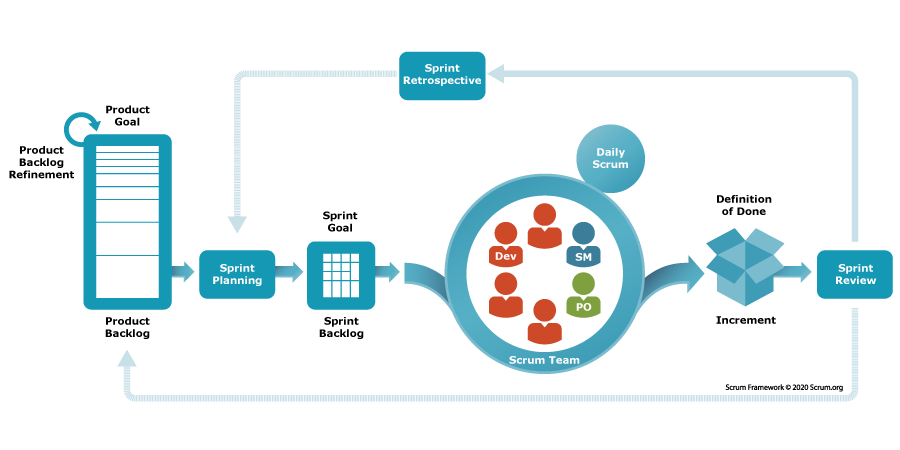
\includegraphics[alt={Rappresentazione del framework Scrum utilizzato in azienda\\ Fonte: scrum.org}, width=0.9\columnwidth]{img/scrum.png}
    \caption[Rappresentazione del \textit{framework} Scrum utilizzato in azienda]{\centering Rappresentazione del \textit{framework} Scrum  utilizzato in azienda \par \textbf{Fonte:} \href{https://www.scrum.org/resources/what-scrum-module}{scrum.org}}
    \label{fig:scrum}
\end{figure}

\section{Tecnologie e strumenti}\label{sec:technologies}

% Lista delle tecnologie utilizzate, descrivendo principalmente le tecnologie utilizzate nella sezione aziendale in cui sono stato inserito, senza menzione di altri progetti a cui non ho partecipato.
\subsection{Tecnologie utilizzate}\noindent
In azienda vengono usate svariate tecnologie, questo è dovuto principalmente dal fatto che vengono svolti più progetti allo stesso tempo. Non avendo familiarità sugli altri progetti, esporrò le tecnologie che furono a me più vicine.
\subsubsection*{Python}\noindent
\textit{Python} è un linguaggio di programmazione ad alto livello, interpretato e di uso generale.
È attualmente il linguaggio più popolare\footnote{Fonte: \href{https://www.tiobe.com/tiobe-index/}{https://www.tiobe.com/tiobe-index/}} al mondo, questo è dovuto dalla semplicità di utilizzo e dal buon supporto di librerie di terze parti, che semplificano ambiti come ad esempio: \textit{web development}, \textit{data science}, \gls{machinelearning} e \textit{scripting} di operazioni ripetitive.
Perciò non stupisce l'utilizzo di questo linguaggio per l'ambito di \textit{machine learning} e per manipolare i \textit{dataset}.
\subsubsection*{TensorFlow}\noindent
\textit{TensorFlow} è una libreria \textit{open-source} sviluppata da \textit{Google} per il \textit{machine learning} e il \gls{deeplearning}.
È una delle librerie più popolari per la creazione e addestramento di modelli basati su tecniche di \textit{machine learning}.
\textit{TensorFlow} integra al suo interno librerie per sfruttare a pieno processori specifici, come ad esempio le \gls{GPU} e le \gls{TPU}, permettendo così di utilizzare risorse computazionali più adeguate, per questo ambito, in modo semplice.
\subsubsection*{Keras}\noindent
Keras è un'altra libreria \textit{open-source} per il \textit{deep learning}, sviluppata per essere semplice e modulare.
Di recente è stata riscritta basandosi su \textit{TensorFlow} e, come quest'ultima, permette di creare e addestrare modelli di intelligenza artificiale, ma rende il processo più rapido e intuitivo.
Keras supporta una variegata tipologia di reti neurali pronte all'uso, come ad esempio reti neurali convoluzionali e ricorrenti, lasciando comunque la possibilità di modificare qualsiasi cosa si voglia adattare meglio alle proprie esigenze.
%Queste caratteristiche rendono questa libreria semplice e potente

% Elenco degli strumenti utilizzati per il supporto i processi, accompagnato da una descrizione del loro scopo e delle loro funzionalità.
\subsection{Strumenti di supporto ai processi}\noindent
\subsubsection*{Jira}\noindent
\textit{Jira} è un software propretario sviluppato da \textit{Atlassian}, è utilizzato come Issue Tracking System (ITS), viene utilizzato per gestire le attività dei vari progetti con la metodologia \textit{Agile}.
All'interno di questo software si possono dedicare delle \textit{board} per i vari \textit{sprint} che vengono svolti.
\begin{figure}[H]
    \centering
    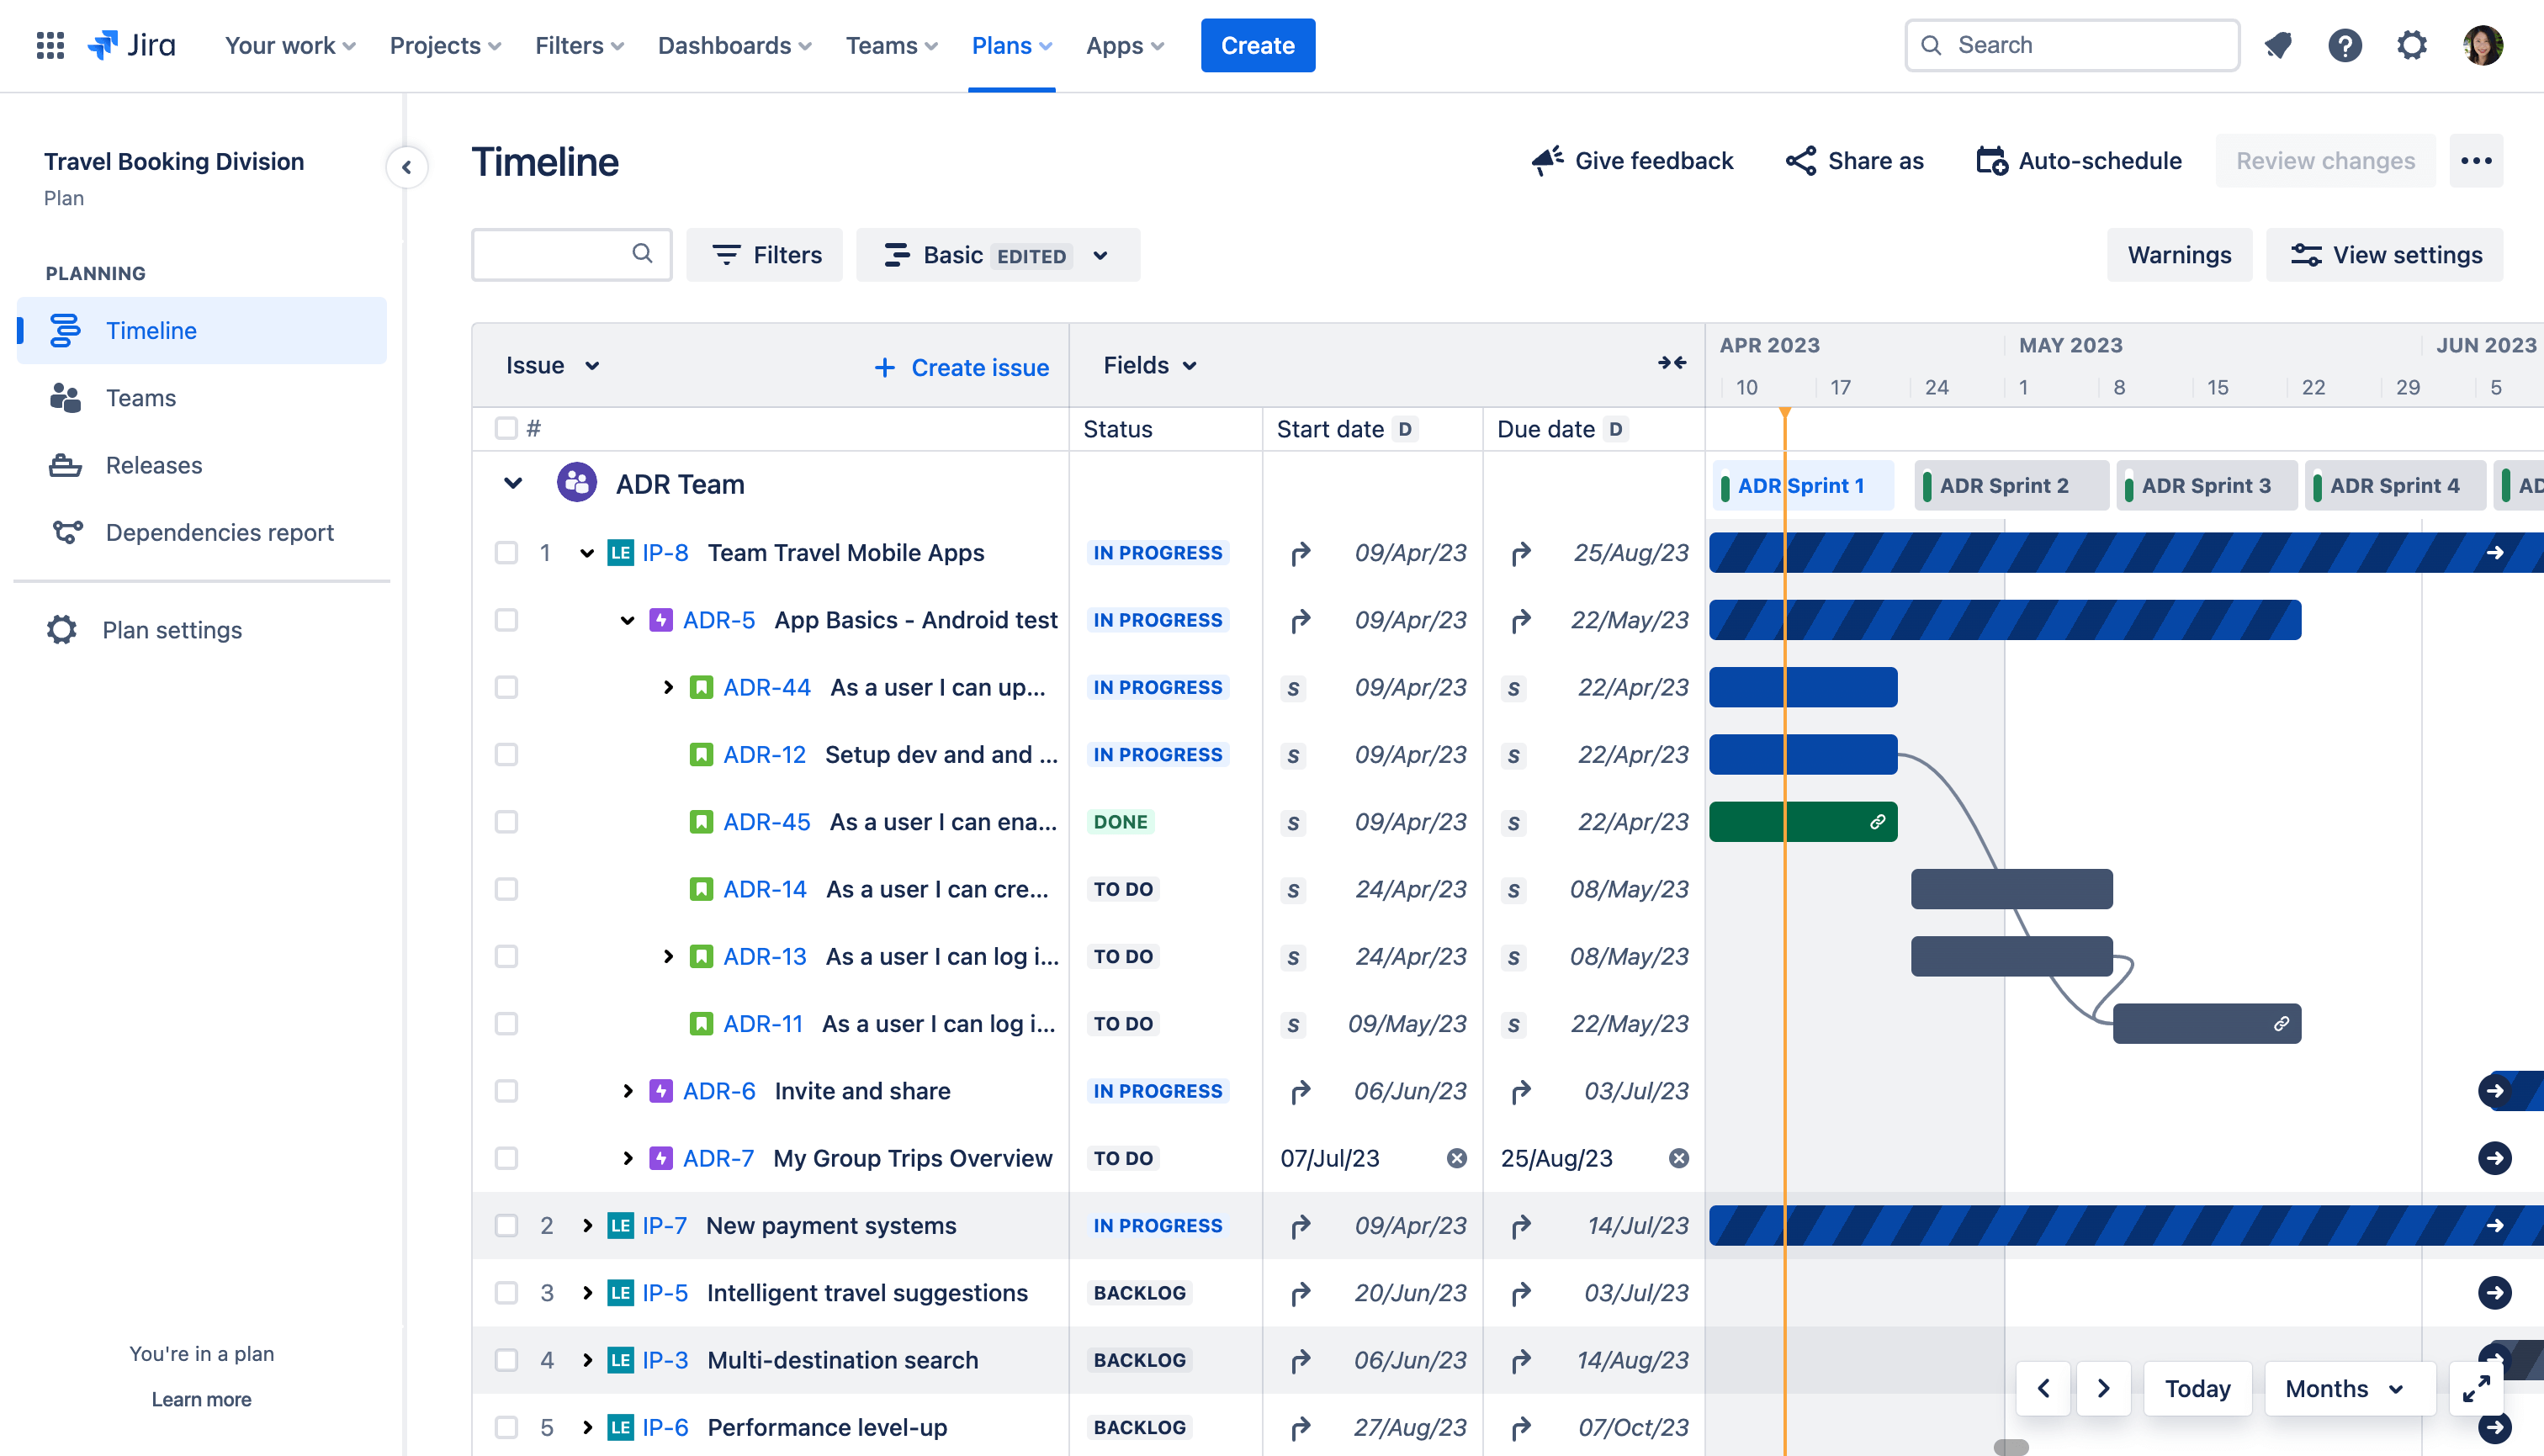
\includegraphics[alt={Esempio di gestione delle attività con \textit{Jira}}, width=0.7\columnwidth]{img/jira.png}
    \caption[Esempio di gestione delle attività con \textit{Jira}]{Esempio di gestione delle attività con \textit{Jira}\\ \textbf{Fonte:} \href{https://www.atlassian.com/it/software/jira/premium}{atlassian.com}}
    \label{fig:jira}
\end{figure}
\subsubsection*{Bitbucket}\noindent
Un'altro software nella suite di \textit{Atlassian} è \textit{Bitbucket}, che viene utilizzato per il controllo di versione e per la gestione del codice sorgente.
Con questo software è possibile creare \textit{repository}, questo spazio permette ai \textit{team} di collaborare in un modo efficiente, avendo anche la disponibilità di utilizzare funzionalità come le \gls{pullrequest}.
\begin{figure}[H]
    \centering
    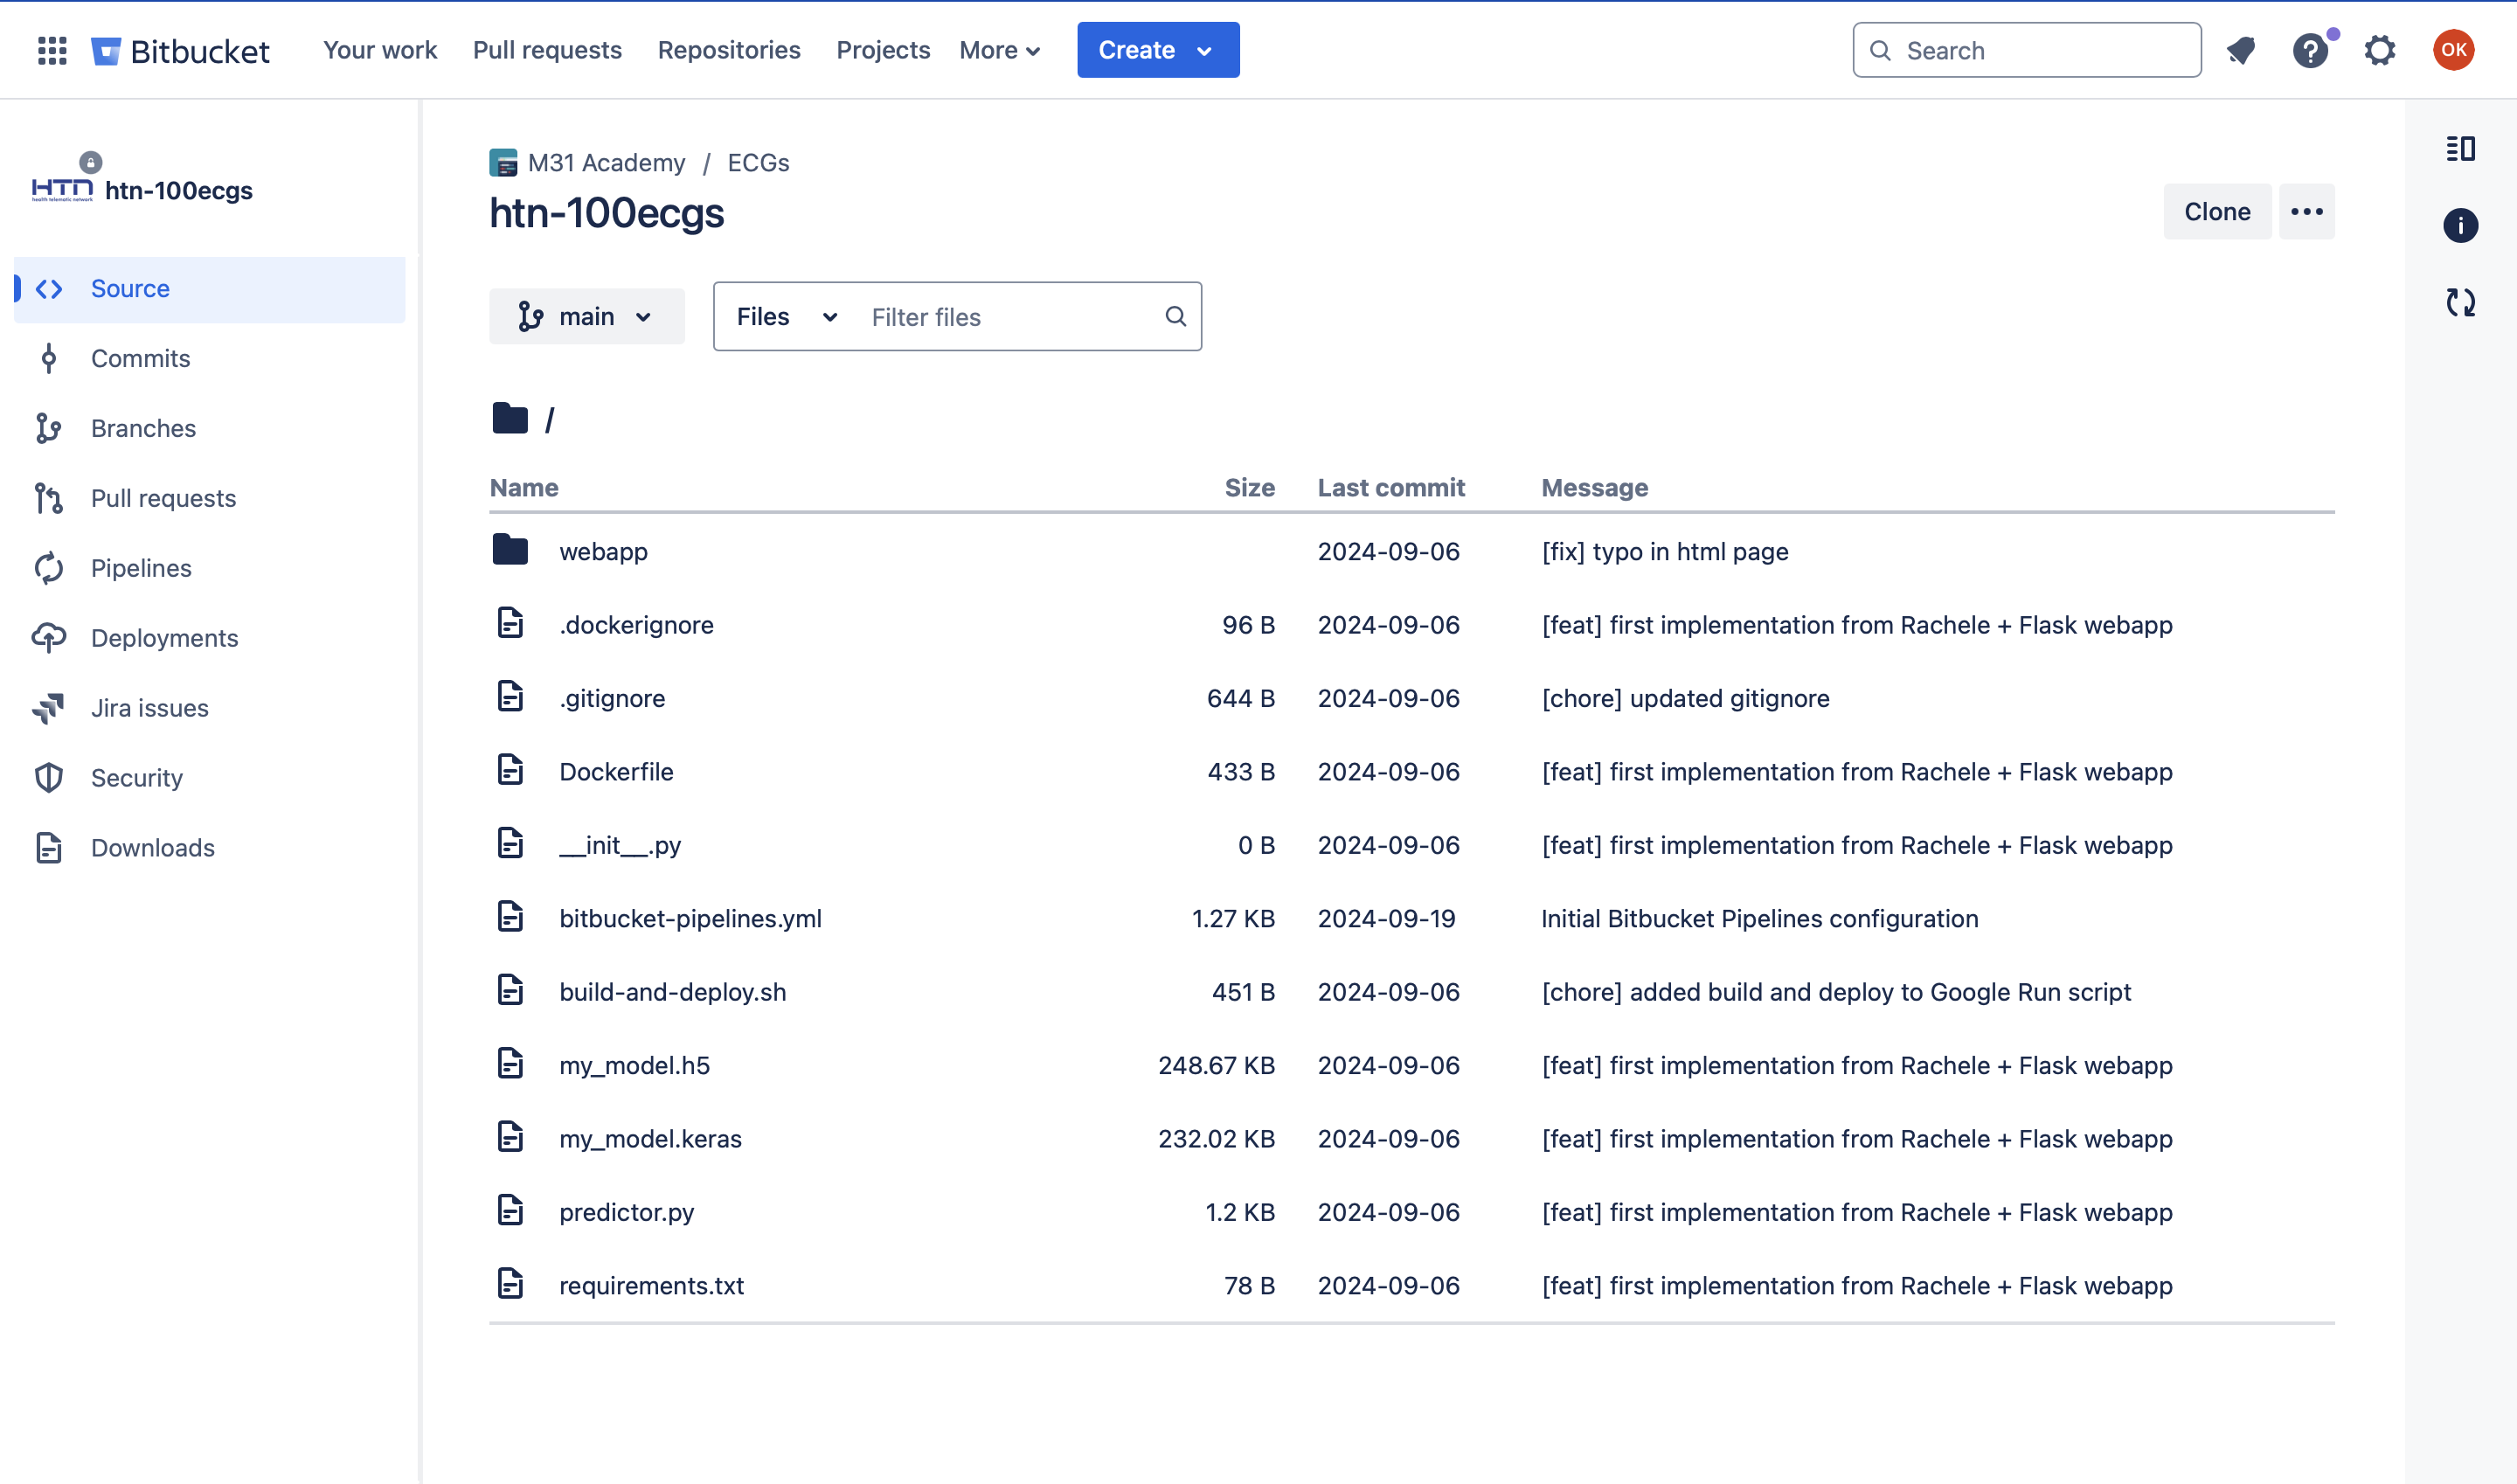
\includegraphics[alt={\textit{Screenshot} di una \textit{repository} in \textit{Bitbucket}}, width=0.9\columnwidth]{img/bitbucket.png}
    \caption{\textit{Screenshot} di una \textit{repository} in \textit{Bitbucket}}
    \label{fig:bitbucket}
\end{figure}
\subsubsection*{Confluence}\noindent
\textit{Confluence} è un'altro software sviluppato da \textit{Atlassian} e viene utilizzato per la gestione della documentazione.
Facendo parte della \textit{suite} di \textit{Atlassian} è ben integrato con le tecnologie precedentemente esposte.
All'interno di questo spazio vengono create documentazioni di prodotti e vari documenti contenenti risorse utili anche internamente.
\begin{figure}[H]
    \centering
    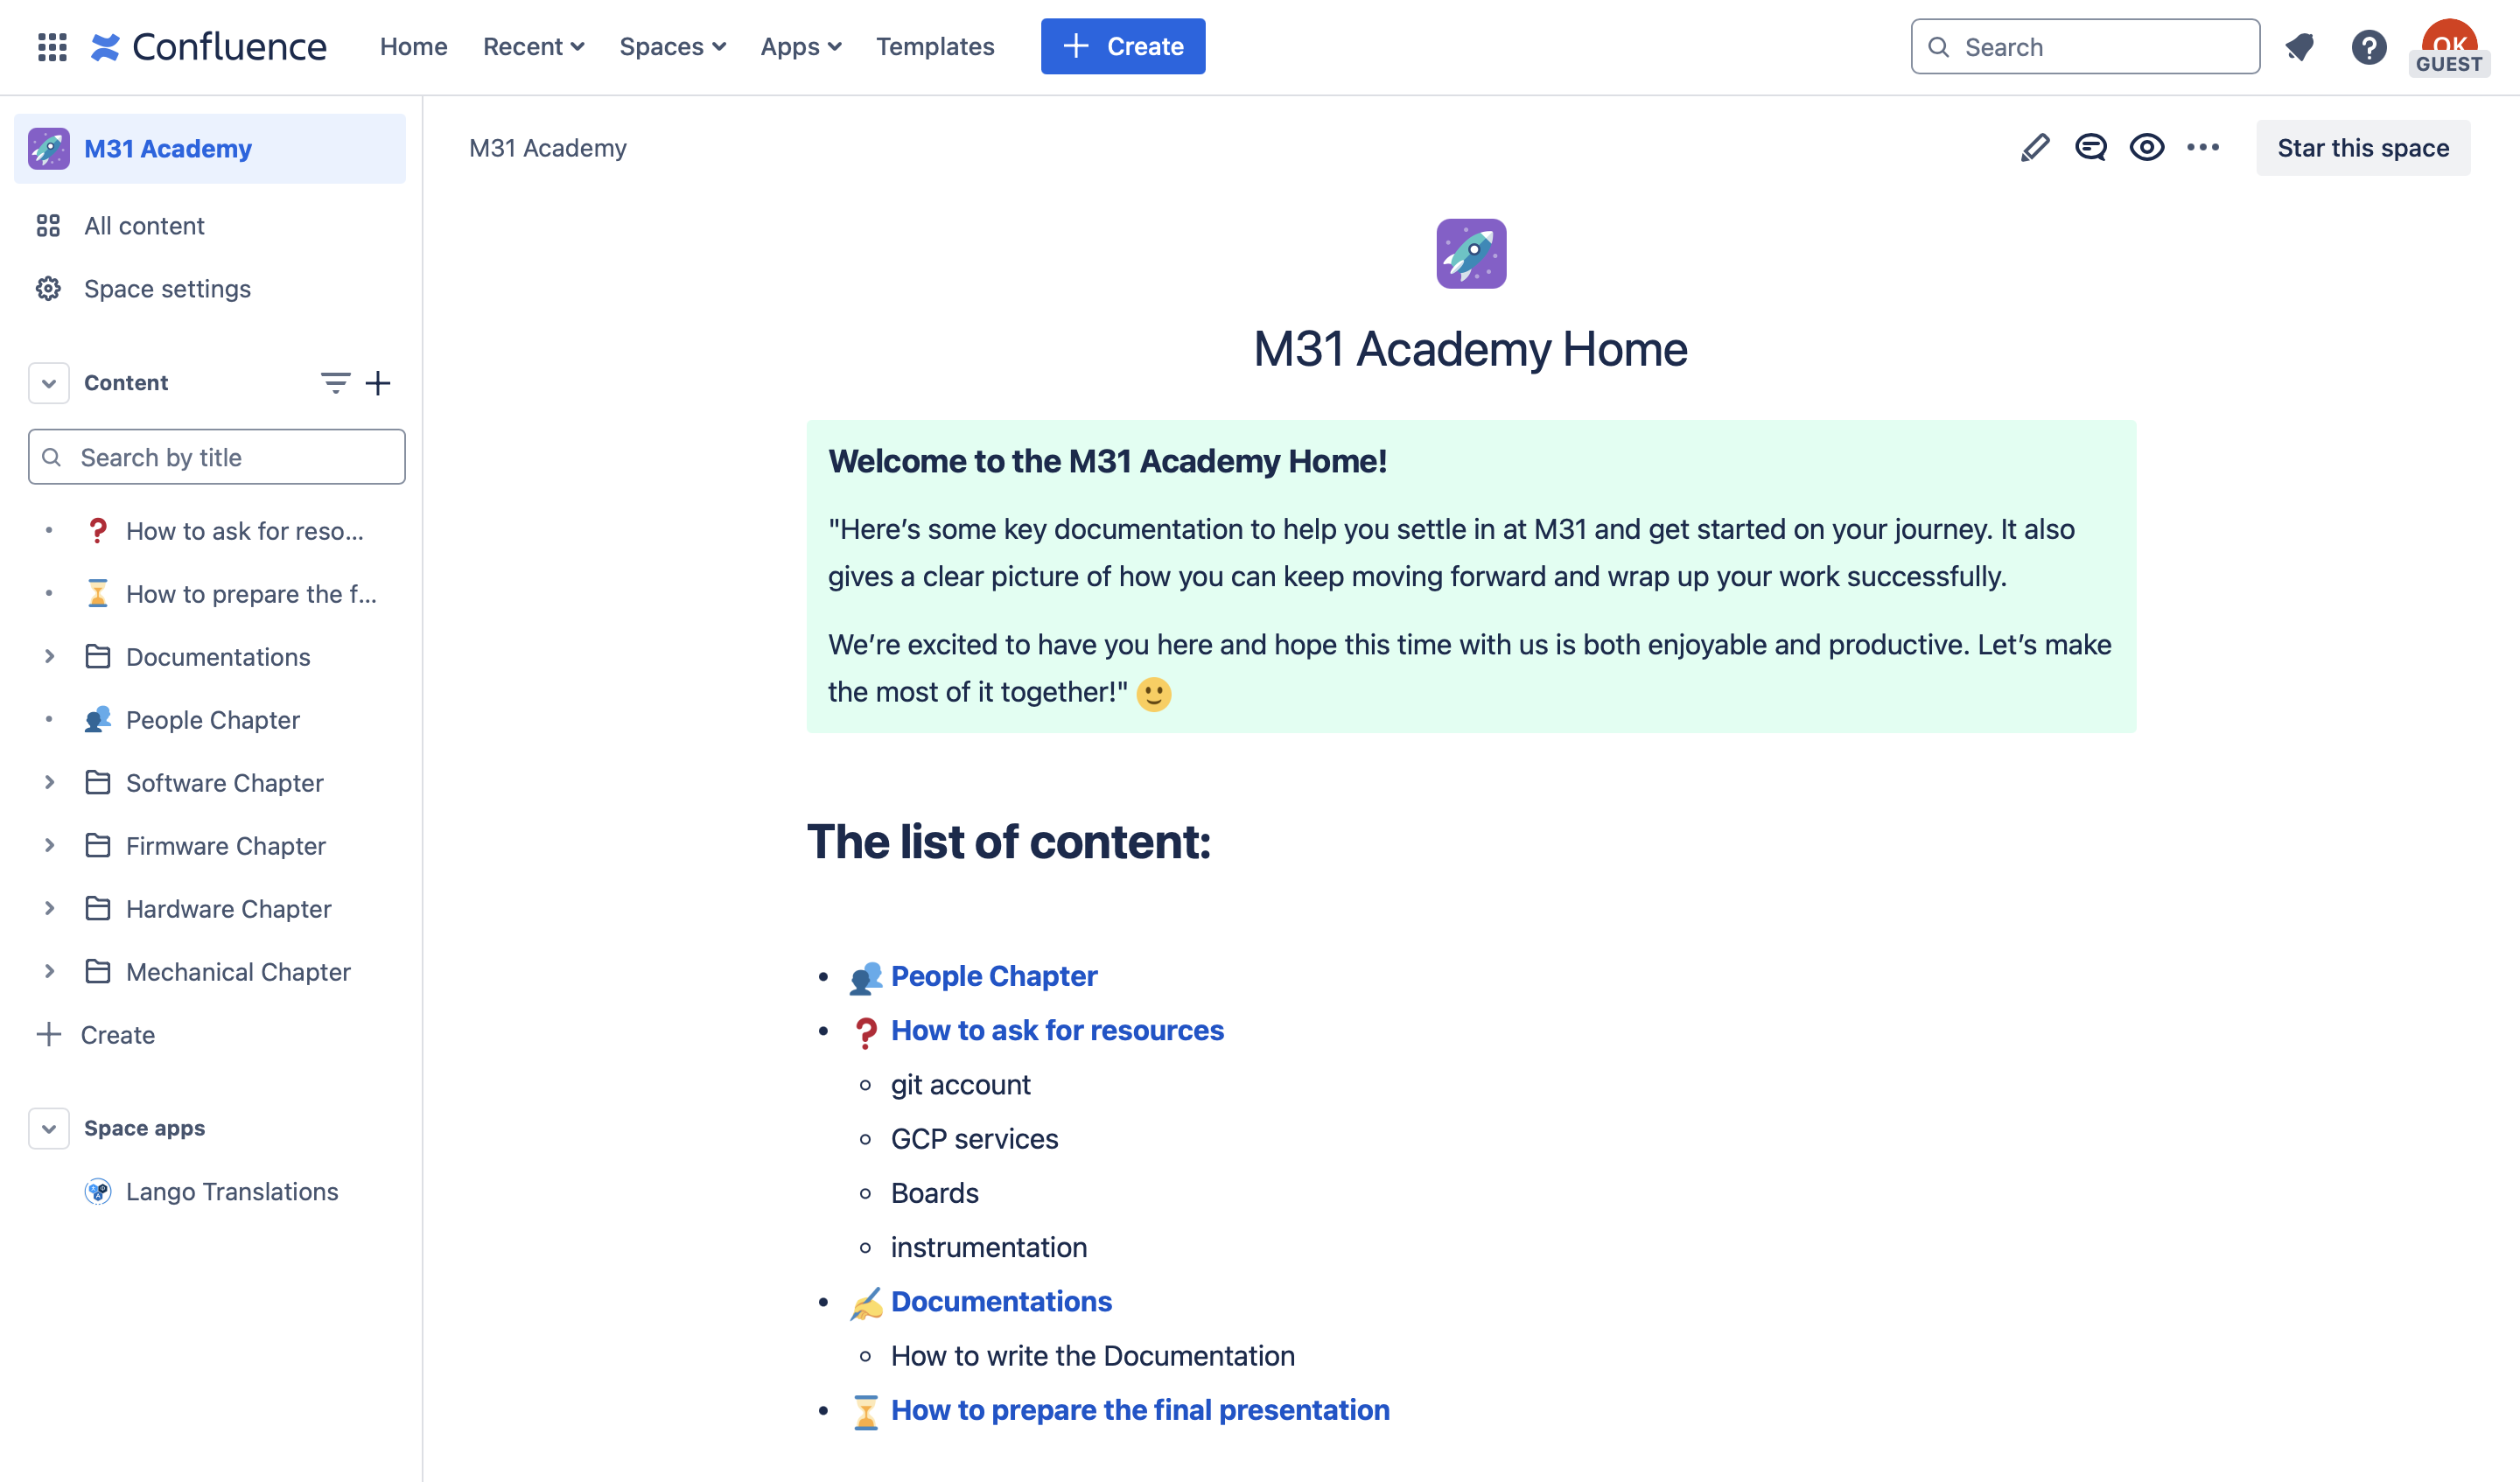
\includegraphics[alt={Pagina principale del \textit{Confluence} di M31 \textit{Academy}}, width=0.9\columnwidth]{img/confluence.png}
    \caption{Pagina principale del \textit{Confluence} di M31 \textit{Academy}}
    \label{fig:confluence}
\end{figure}
\subsubsection*{Microsoft Teams}\noindent
L'applicativo che viene utilizzato per comunicare è \textit{Microsoft Teams}. Questo software sviluppato da \textit{Microsoft} permette di comunicare, con singoli individui o con gruppi di persone, sia tramite messaggi testuali che tramite videochiamate.
Può essere usato anche per trasferimenti di piccoli file, ed è la prima opzione per comunicare con i membri dei team che lavorano da remoto.
\begin{figure}[H]
    \centering
    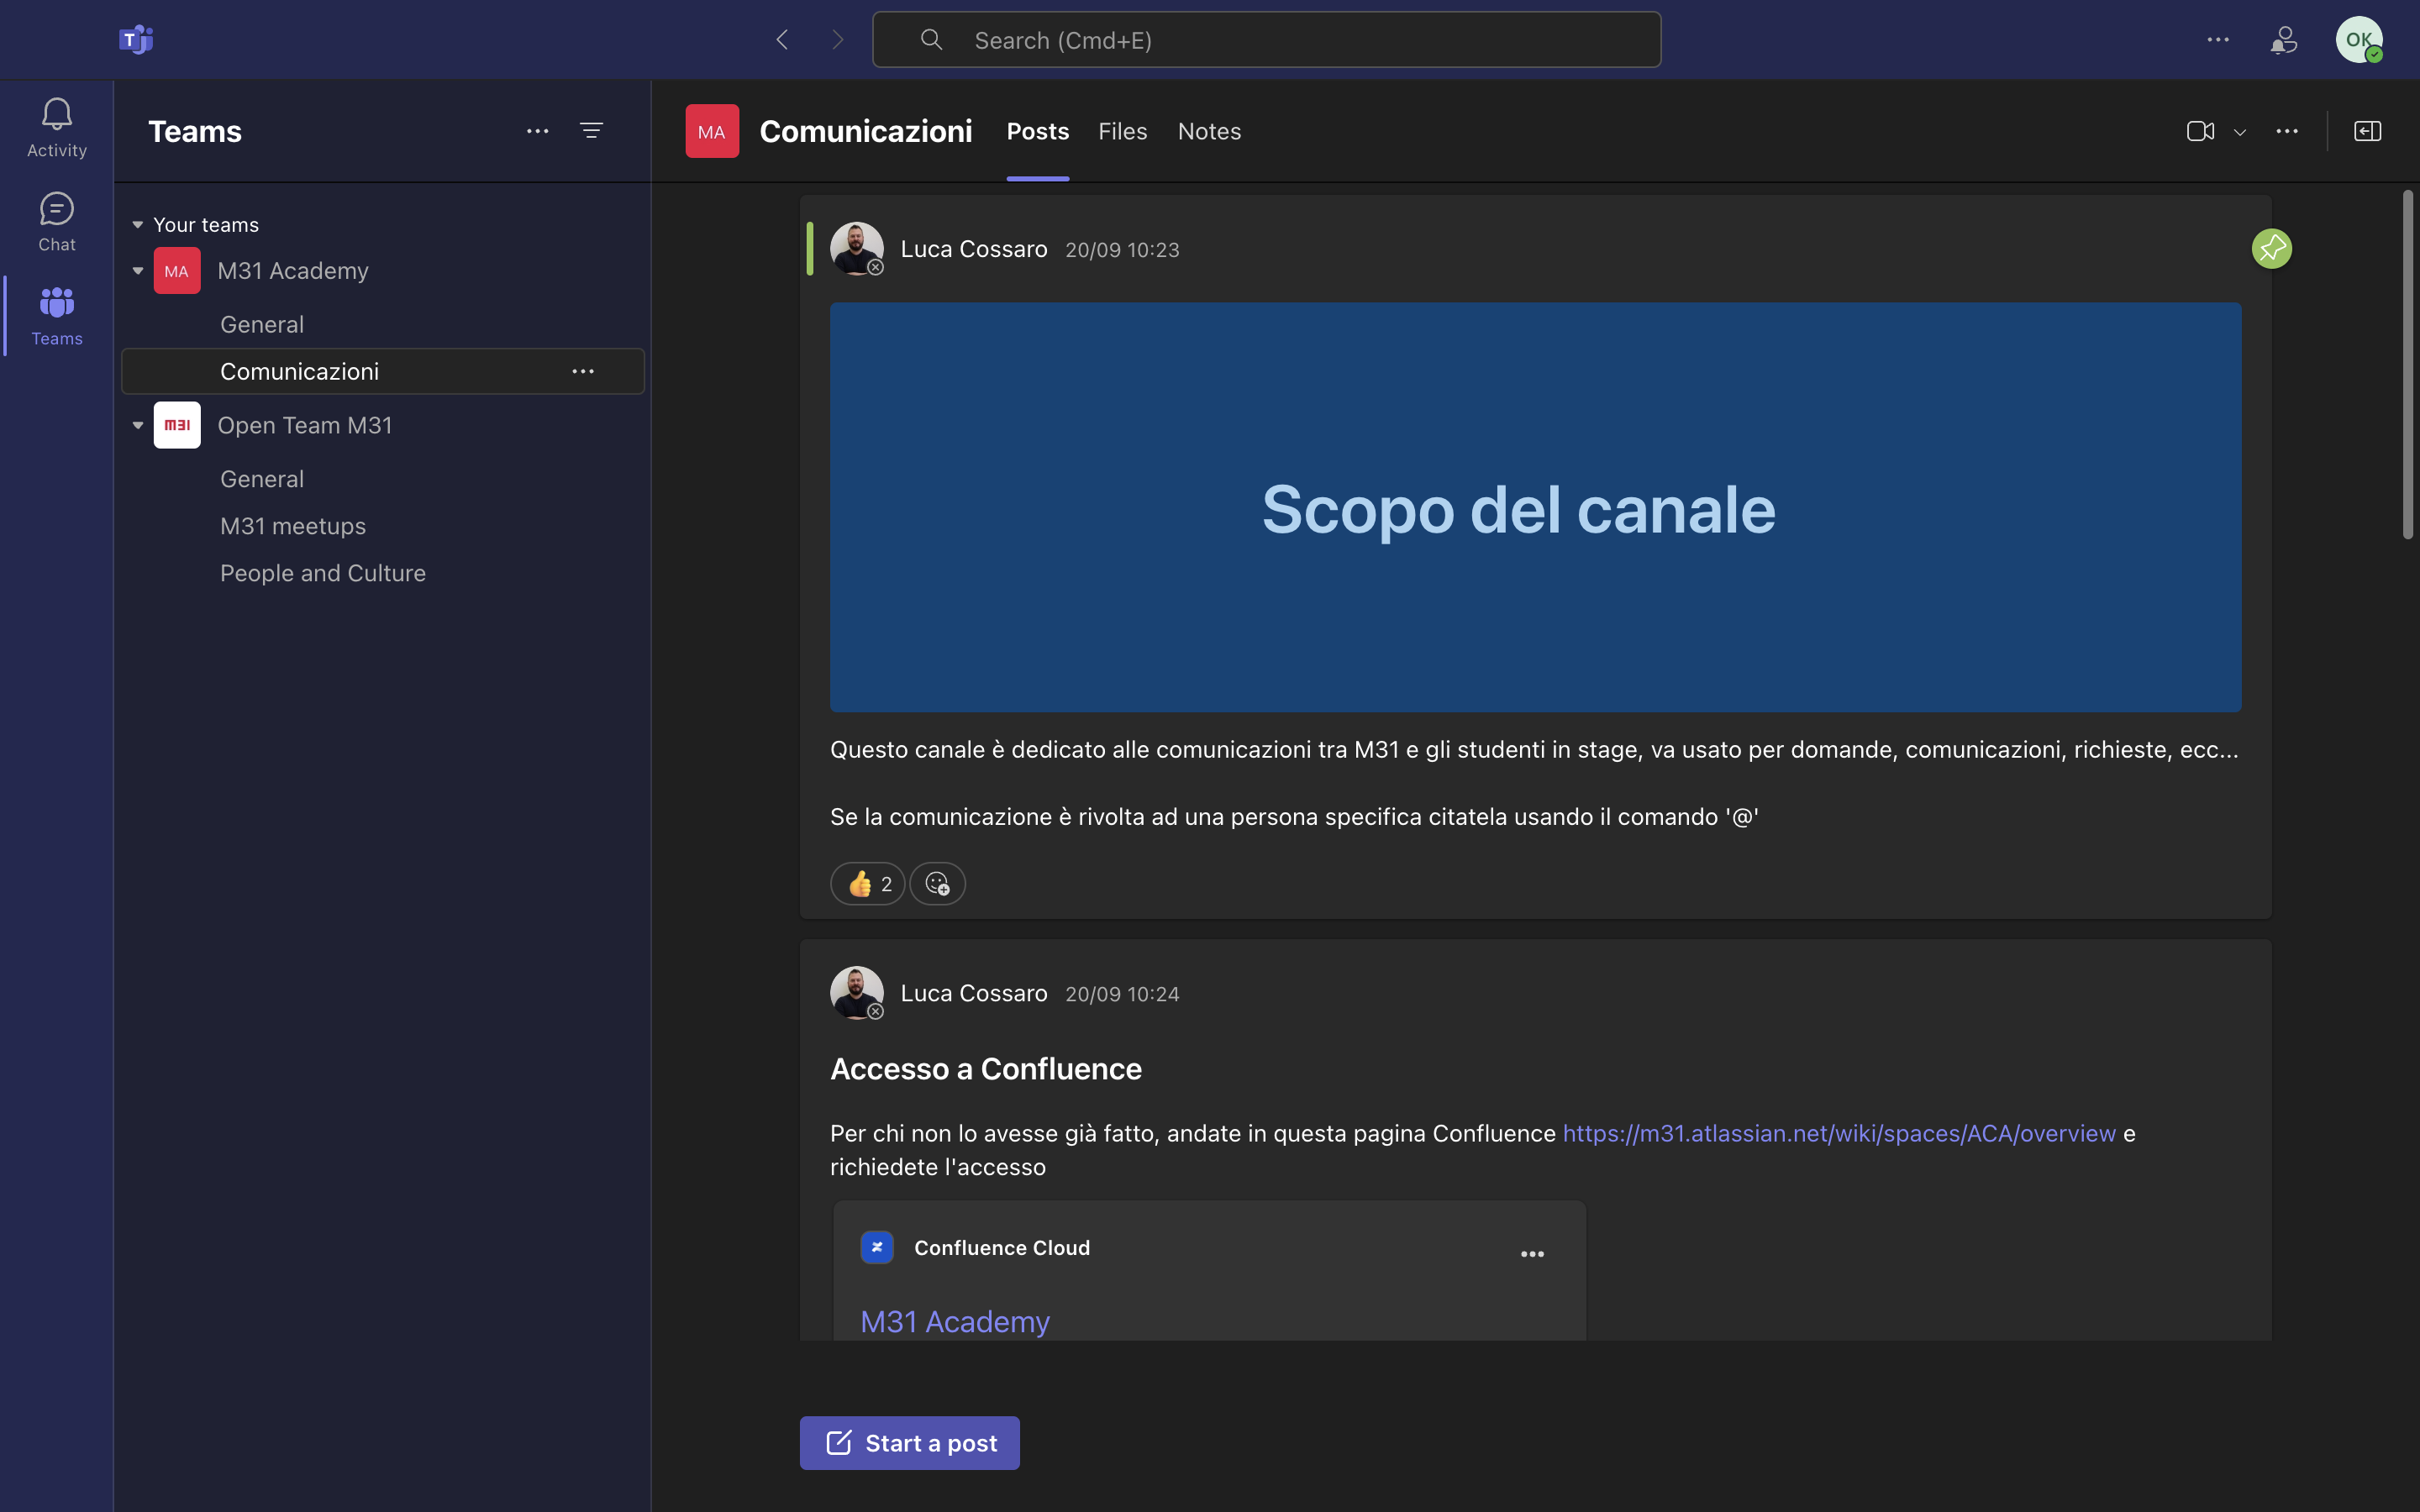
\includegraphics[alt={\textit{Screenshot} di un canale di comunicazione di M31 \textit{Academy}}, width=0.9\columnwidth]{img/microsoft-teams.png}
    \caption{\textit{Screenshot} di un canale di comunicazione di M31 \textit{Academy}}
    \label{fig:teams}
\end{figure}

% In questa sezione viene descritta come l'azienda si approccia con l'innovazione.
\section{Propensione all'innovazione}\label{sec:innovation}\noindent
M31 si interessa parecchio all'innovazione e questo lo si può vedere dalla filosofia con cui intraprende nuovi progetti di lavoro, come già menzionato nella sezione introduttiva \ref{sec:the-company}, i progetti che svolge sono tutti con lo scopo di portare progresso nei settori in cui si specializza.
Inoltre, durante lo svolgimento del mio tirocinio, ho potuto assistere ad un \textit{meeting} plenario che viene svolto periodicamente, nel quale ho potuto vedere in quali settori è l'azienda è intenzionata ad esplorare in futuro, sia dal lato della dirigenza che dal lato dei dipendenti.
    \chapter{\textit{Stage} proposto}
\label{chap:stage-proposto}

\section{Gestione aziendale degli \textit{stage}}\label{sec:stage-management}\noindent
% \texttt{Descrizione di come sono visti e gestiti in generale gli stage all'interno dell'azienda.}
M31 mostra molto interesse verso la creazione di rapporti con le nuove generazioni, questo avviene in diversi modi: tramite la M31 \textit{Academy} e tramite la partecipazione ai progetti di ``Ingegneria del \textit{Software}'' della laurea triennale di informatica, come azienda proponente.\\
M31 \textit{Academy} è una sorta di settore aziendale dedicato alla realizzazione di progetti con studenti universitari o neo-laureati. Ora come ora, l'azienda sta svolgendo progetti solo con studenti universitari, che prendono il ruolo di stagisti, perciò passo a descrivere meglio come essi vengono gestiti.\\
L'influsso di stagisti è principalmente dovuto alla partecipazione dell'azienda allo \textit{STAGE-IT}, un evento promosso da Confindustria Veneto Est e l'Università di Padova, dove gli studenti vengono introdotti a tre progetti che possono svolgere in azienda. M31 però offre una lista più numerosa di progetti, che vengono esposti quando gli studenti contattano direttamente l'azienda.
Questi progetti, essendo numerosi, possono essere di vario tipo: alcuni pongono gli stagisti in un progetto su cui l'azienda sta già lavorando, mentre altri progetti, come quello che ho scelto io, servono all'azienda per esplorare nuove tecnologie o per prepararsi per un progetto aziendale che non ha ancora avuto modo di iniziare.

\section{Descrizione progetto}\label{sec:project-description}\noindent
% \texttt{Esposizione del problema affrontato dal mio progetto di stage.}
Il progetto che ho affrontato in azienda consisteva nella realizzazione di un'applicazione per l'analisi di dati tramite tecniche di \gls{machinelearning} e di \gls{deeplearning}; in particolare, per l'analisi di segnali elettrocardiografici.\\
Questo progetto di \textit{stage} serviva all'azienda per prepararsi ad un progetto che si aspettano di affrontare in futuro, collaborando insieme ad un'azienda con cui sono attualmente in comunicazione.\\
Questo progetto vede come \textit{focus} principale la gestione di grandi quantità di dati. Questi dati, facenti parte di un \gls{dataset}, devono essere gestiti correttamente e nel modo più efficiente possibile all'interno di un sistema capace di effettuare addestramenti di \glslink{neuralnetwork}{reti neurali artificali}, ovvero di modelli che cercano di replicare il funzionamento del cervello umano.\\
In secondo luogo, il progetto vede anche l'effettivo addestramento e valutazione di vari tipi di reti neurali artificiali, sia con lo scopo di testare, che di esplorare quali sono le tecniche migliori per l'analisi di elettrocardiogrammi.
\begin{figure}[H]
    \centering
    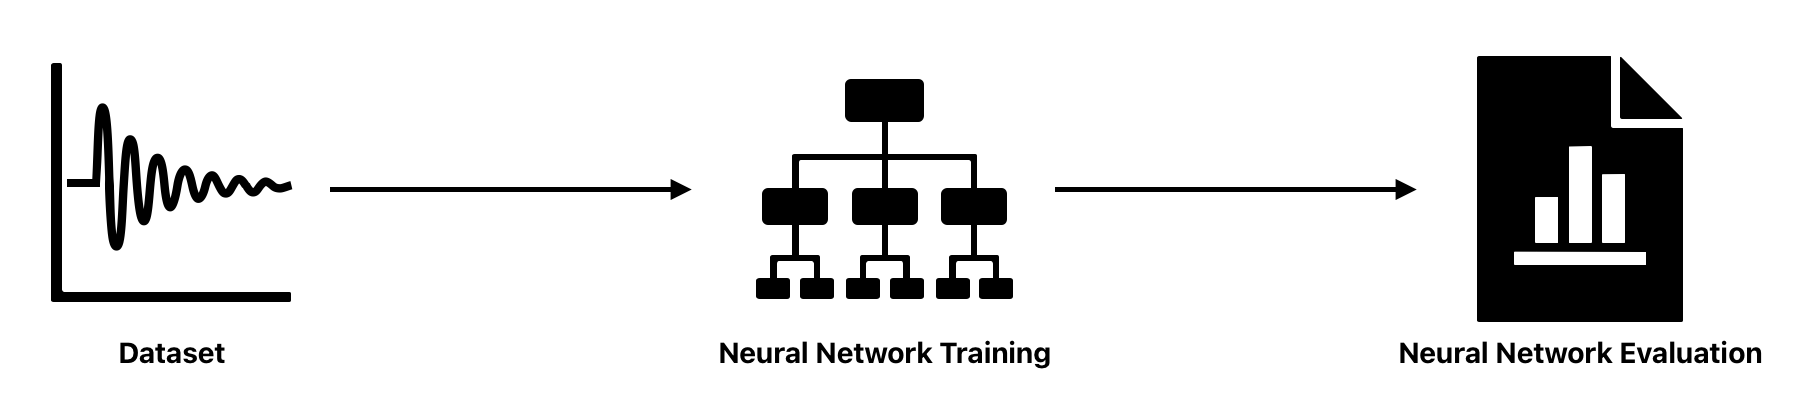
\includegraphics[alt={Rappresentazione dei punti principali del progetto}, width=0.9\columnwidth]{img/desc_proj.png}
    \caption{\centering Rappresentazione dei punti principali del progetto}
    \label{fig:desc-proj}
\end{figure}

\section{Obiettivi}\label{sec:objectives}\noindent
%\texttt{Lista degli obiettivi da completare che riguardano il prodotto del mio operato durante lo stage, quindi quello che l'azienda vuole ottenere.}\\
Il progetto di \textit{stage} era caratterizzato da degli obiettivi richiesti dall'azienda, ognuno di essi era contrassegnato con una certa importanza; questa può rientrare in una dei tre seguenti tipi:
\begin{itemize}
    \item \textbf{Obbligatorio:} indica un obiettivo primario richiesto dal committente, il suo completamento non è negoziabile
    \item \textbf{Desiderabile:} indica un obiettivo non vincolante o strettamente necessario, ma dal riconoscibile valore aggiunto
    \item \textbf{Facoltativo:} indica un obiettivo facoltativo, che rappresenta valore aggiunto e non strettamente competitivo
\end{itemize}
Nella tabella \ref{tab:obiettivi}, definita successivamente, vengono esposti i vari obiettivi aziendali che sono stati imposti per il completamento del progetto:
\begin{center}
    \rowcolors{1}{}{tableGray}
    \begin{longtable}{|p{10.5cm}|p{2.5cm}|}
    \hline
    \multicolumn{1}{|c|}{\textbf{Obiettivo}} & \multicolumn{1}{c|}{\textbf{Importanza}}\\ 
    \hline 
    \endfirsthead
    \rowcolor{white}
    \multicolumn{2}{c}{{\bfseries \tablename\ \thetable{} -- Continuo della tabella}}\\
    \hline
    \multicolumn{1}{|c|}{\textbf{A}} & \multicolumn{1}{c|}{B}\\ \hline 
    \endhead
    \hline
    \rowcolor{white}
    \multicolumn{2}{|r|}{{Continua nella prossima pagina...}}\\
    \hline
    \endfoot
    \endlastfoot 
    
    Studio delle tecnologie e del contesto specifico & \multicolumn{1}{c|}{Obbligatorio} \\
    \hline
    Creazione di un dataset appropriato e di tecniche per la sua gestione & \multicolumn{1}{c|}{Obbligatorio} \\
    \hline
    Implementazione in \textit{Python} degli algoritmi basati su tecniche di \textit{deep learning} & \multicolumn{1}{c|}{Obbligatorio} \\
    \hline
    Valutazione dell'esecuzione  degli algoritmi & \multicolumn{1}{c|}{Obbligatorio} \\
    \hline
    Realizzazione di \textit{unit test} & \multicolumn{1}{c|}{Desiderabile} \\
    \hline
    Idee o suggerimenti su come migliorare in futuro la performance del'applicativo' & \multicolumn{1}{c|}{Facoltativo} \\
    \hline
    \hiderowcolors
    \caption{Lista dei vari obiettivi aziendali.}
    \label{tab:obiettivi}
    \end{longtable}
\end{center}

\section{Vincoli}\label{sec:restrictions}

\subsection{Vincoli tecnologici}\noindent
% \texttt{Vengono indicati i vari vincoli sulle tecnologie utilizzate.}
Per i vincoli tecnologici, alcune delle tecnologie mi sono state imposte per la realizzazione di questo progetto.
Queste tecnologie sono relative all'addestramento dei modelli di intelligenza artificiale, dove ho usato Keras.
Utilizzando questa tecnologia, però, si è inoltre obbligati a fare uso di \textit{Python} e, per aumentare la semplicità di installazione dei pacchetti di questo linguaggio di programmazione, si è imposto anche l'uso di \textit{Conda}, un sistema per la gestione di pacchetti e \gls{environment}, che ha permesso l'installazione di ciò che era necessario senza troppi intoppi.

\subsection{Vincoli temporali}\label{subsec:time-restrictions}\noindent
% \texttt{Viene menzionato il limite di tempo dello stage.}
Per la sua natura, il tirocinio curricolare ha un limite di tempo: ovvero deve essere dalle 300 alle 320 ore di lavoro, e non è possibile sforare 40 ore settimanalmente.
Per lavorare al progetto, lo \textit{stage} è stato distribuito in giornate lavorative da 8 ore ciascuno, per un totale di all'incirca 38 giorni.

\subsection{Vincoli organizzativi}\noindent
% \texttt{Descrizione dei vincoli per il corretto mantenimento dell'andamento dello stage.}
Per il corretto svolgimento del tirocinio curricolare, sono stati presi alcuni accorgimenti.\\
In primis, svolgevo periodicamente dei \textit{meeting} con il mio \textit{tutor} aziendale, nei quali esponevo le attività svolte da me durante l'ultimo periodo, in modo da far sì che l'avanzamento del progetto si allineasse con gli obiettivi imposti in modo corretto.\\
In secundis, ogni cinque giorni lavorativi dovevo mandare una \textit{email} al mio relatore di tesi, indicando quali attività erano previste da svolgere durante la settimana lavorativa passata, e come esse sono state svolte rispetto alle aspettative.

\section{Motivazione della scelta}\label{sec:choice-motivation}\noindent
% \texttt{Esposizione della motivazione per cui ho scelto questo specifico progetto di stage e non qualche altra opzione.}\\
% \texttt{Vengono inoltre esposti gli obiettivi imposti personalmente che riguardano la mia crescita professionale.}
Sono venuto a conoscenza di M31 attraverso l'evento \textit{STAGE-IT}, un'iniziativa che mi ha dato la possibilità di incontrare, in un singolo posto, diverse aziende e le loro proposte di \textit{stage}.
Tra le aziende presenti, M31 era una di quelle che mi ha interessato di più, questo perchè avevo un maggiore interesse a svolgere un progetto che utilizzava, in qualche maniera, l'intelligenza artificiale.\\
M31 durante l'evento \textit{STAGE-IT} aveva proposto un tema di \textit{machine learning} in ambito di \gls{computervision}, che ero intenzionato nel svolgere quando stavo contattando l'azienda, ma vedendo la lista aggiornata dei progetti di \textit{stage} offerti, ho deciso di scegliere un secondo progetto, sempre di intelligenza artificiale, ma in ambito biomedico, questo perchè le tecniche utilizzate per questo specifico ambito mi sarebbero state nuove.\\
% Oltre all'obiettivo di espandere le mie conoscenze nell'argomento trattato nel progetto, avevo altri obiettivi personali, come ad esempio: capire come opera effettivamente un'azienda di questo settore, essendo la mia prima esperienza lavorativa in questo ambito, oppure di migliorare l'abilità di \textit{problem solving}.
Gli obiettivi personali che mi sono posto prima di svolgere questo tirocinio possono essere rappresentati nella seguente lista:
\begin{itemize}
    \item \textbf{Approfondimento tecnico:} avendo parecchio interesse verso l'intelligenza artificiale, ero intenzionato, con questo \textit{stage}, nell'approfondire questo argomento svolgendo un progetto con un'applicazione in questo ambito, per me nuova. Questo obiettivo è dovuto anche dal fatto che sono intenzionato nel proseguire gli studi con la laurea magistrale.
    \item \textbf{Capire l'ambiente lavorativo:} essendo la mia prima esperienza lavorativa in questo settore, ero incuriosito da come, effettivamente, le aziende operano internamente. Non solo apprendere le metodologie aziendali, ma anche la cultura lavorativa.
    \item \textbf{\textit{Problem solving}:} migliorare nell'abilità di risolvere problemi, in modo da trovare soluzioni efficienti a vari problemi a diverse sfide.
\end{itemize}
    \chapter{Svolgimento dello \textit{stage}}
\label{chap:svolgimento-stage}

\section{Pianificazione delle attività}\label{sec:activity-planning}\noindent
% \texttt{Esposizione di come sono state pianificate le attività.}
Come già menzionato nella sezione \ref{subsec:time-restrictions}, il progetto di \textit{stage} è stato suddiviso in diverse giornate lavorative.
Le giornate sono suddivise in otto settimane, ciascuna delle quali prevede delle attività da svolgere, decise all'inizio dello svolgimento del tirocinio, basandosi sul piano di lavoro redatto prima dell'inizio dello stesso.
Di seguito vengono esposte le varie attività per settimana:
\begin{itemize}
    \item \textbf{Prima settimana:}
        \begin{itemize}
            \item Studio del problema specifico dell'analisi di elettrocardiogrammi
            \item Definizione delle \textit{user story}
        \end{itemize}
    \item \textbf{Seconda settimana:}
        \begin{itemize}
            \item Formazione e ricerca di tecniche di \textit{deep learning} specifiche per il problema di analisi di serie temporali
            \item Studio del \textit{dataset} pubblico PTB-XL
        \end{itemize}

    \newpage

    \item \textbf{Terza settimana:}
        \begin{itemize}
            \item Ricerca e analisi delle tecniche di \textit{deep learning} specifiche per il problema affrontato
            \item Analisi e confronto del \textit{dataset} pubblico con le caratteristiche del \textit{dataset} privato
            \item Realizzazione di un primo prototipo dell'applicazione di addestramento
        \end{itemize}
    \item \textbf{Quarta settimana:}
        \begin{itemize}
            \item Modifica e riduzione del \textit{dataset} rispettando i requisiti imposti
            \item Implementazione della \textit{Sequential} \gls{api} di Keras
            \item Prima implementazione del caricamento ottimizzato del \textit{dataset}
        \end{itemize}
    \item \textbf{Quinta settimana:}
        \begin{itemize}
            \item Implementazione della \textit{Functional} API di Keras
            \item Completamento dell'implementazione del caricamento ottimizzato del \textit{dataset}
            \item \textit{Testing} dell'implementazione della \textit{Sequential} API
        \end{itemize}
    \item \textbf{Sesta settimana:}
        \begin{itemize}
            \item Implementazioni di tecniche di \gls{downsampling} e di \gls{preprocessing}
            \item \textit{Testing} dell'implementazione della \textit{Functional} API
        \end{itemize}
    \item \textbf{Settima settimana:}
        \begin{itemize}
            \item \textit{Testing} dell'intero applicativo
            \item Svolgimento di vari addestramenti di reti neurali artificiali
        \end{itemize}
    \item \textbf{Ottava settimana:}
        \begin{itemize}
            \item Valutazione dell'applicazione creata
            \item Realizzazione della presentazione finale in azienda
        \end{itemize}
\end{itemize}

\section{Analisi dei requisiti}\label{sec:analysis}\noindent
% \texttt{Descrizione dell'attività di analisi dei requisiti.}
Per garantire che il prodotto finale soddisfi le aspettative e gli obiettivi, è necessario analizzare a fondo le varie esigenze e aspettative degli \textit{stakeholder} che esso dovrà soddisfare.
Per fare ciò, ho utilizzato l'approccio delle \textit{user story}, ovvero varie descrizioni semplici delle funzionalità dal punto di vista dell'utente.\\
Le \textit{user story} vengono raccolte e identificate in una lista tramite un codice, esso è strutturato nel seguente modo:
\begin{center}
    \textbf{US-[Numero incrementale]}
\end{center}\noindent
Queste \textit{user story} sono state approvate con il \textit{tutor} e ognuna di essa è mandatoria.
% Technically the code shoud use US and not just U
\begin{center}
    \rowcolors{1}{}{tableGray}
    \begin{longtable}{|p{2.5cm}|p{10.5cm}|}
    \hline
    \multicolumn{1}{|c|}{\textbf{Identificatore}} & \multicolumn{1}{c|}{\textbf{\textit{User story}}}\\ 
    \hline 
    \endfirsthead
    \rowcolor{white}
    \multicolumn{2}{c}{{\bfseries \tablename\ \thetable{} -- Continuo della tabella}}\\
    \hline
    \multicolumn{1}{|c|}{\textbf{Identificatore}} & \multicolumn{1}{c|}{\textbf{\textit{User story}}}\\ \hline 
    \endhead
    \hline
    \rowcolor{white}
    \multicolumn{2}{|r|}{{Continua nella prossima pagina...}}\\
    \hline
    \endfoot
    \endlastfoot
    
    \multicolumn{1}{|c|}{US-1} & Come utente, voglio che il \textit{dataset} pubblico PTB-XL venga usato per svolgere addestramenti di reti neurali artificiali, così che io possa provare diverse strutture nell'ambito dell'analisi di segnali elettrocardiografici. \\
    \hline
    \multicolumn{1}{|c|}{US-2} & Come utente, voglio che il \textit{dataset} venga caricato nella fase di \textit{training} senza sforare i limiti della RAM, in modo da permettere addestramenti di reti neurali artificiali con \textit{dataset} di qualsiasi dimensioni \\
    \hline
    \multicolumn{1}{|c|}{US-3} & Come utente, voglio che i parametri per l'addestramento di reti siano in un singolo posto, in modo da facilitare il processo di addestramento di nuovi modelli basati su nuove strutture \\
    \hline
    \multicolumn{1}{|c|}{US-4} & Come utente, voglio che la rete neurale artificiale abbia come come input aggiuntivo, oltre al segnale elettrocardiografico, anche altre informazioni come età e peso del paziente, in modo da aumentare i risultati dei modelli creati con i vari addestramenti \\
    \hline
    \multicolumn{1}{|c|}{US-5} & Come utente, voglio che ci sia la possibilità di fare \textit{preprocessing}, in modo da applicare funzioni per estrarre \textit{features} \\
    \hline
    \multicolumn{1}{|c|}{US-6} & Come utente, voglio che ci sia la possibilità di applicare \textit{downsampling}, in modo da ridurre la dimensione dei dati in entrata \\
    \hline
    \multicolumn{1}{|c|}{US-7} & Come utente, voglio che i modelli addestrati diano in output due classi, in modo da capire se il paziente è sano o no \\
    \hline
    \multicolumn{1}{|c|}{US-8} & Come utente, voglio che i modelli addestrati diano in output cinque classi, in modo da capire in quale delle superclassi del \textit{dataset} fa parte la diagnosi dell'elettrocardiogramma \\
    \hline
    \multicolumn{1}{|c|}{US-9} & Come utente, voglio che i modelli addestrati possano essere confrontati con i \textit{file} del dataset privato, in modo da mantenere una compatibilità tra i due \textit{dataset} \\
    \hline
    \multicolumn{1}{|c|}{US-10} & Come utente, voglio che il programma crei una \gls{confusionmatrix}, in modo da valutare oggettivamente la prestazione del modello addestrato \\
    \hline
    \multicolumn{1}{|c|}{...} & \multicolumn{1}{|c|}{...}  \\
    \hline
    \multicolumn{1}{|c|}{US-19} & Come utente, voglio che il programma crei un grafico di \gls{confidence} usando i dati del \textit{dataset} privato, in modo da valutare oggettivamente la prestazione del modello addestrato \\
    \hline
    \multicolumn{1}{|c|}{US-20} & Come utente, voglio che l'applicazione salvi ogni metrica e modelli creati in una \textit{directory} dedicata, in modo da poter salvare ogni addestramento svolto e dare la possibilità di confrontare i risultati se ce ne fosse bisogno \\
    \hline
    \hiderowcolors
    \caption{Tabella contenente le varie \textit{user story}.}
    \label{tab:user-stories}
    \end{longtable}
\end{center}

\section{Progettazione}\label{sec:design}\noindent
% \texttt{Descrizione dell'attività di progettazione.}

\subsection{Visione d'insieme}
\begin{figure}[H]
    \centering
    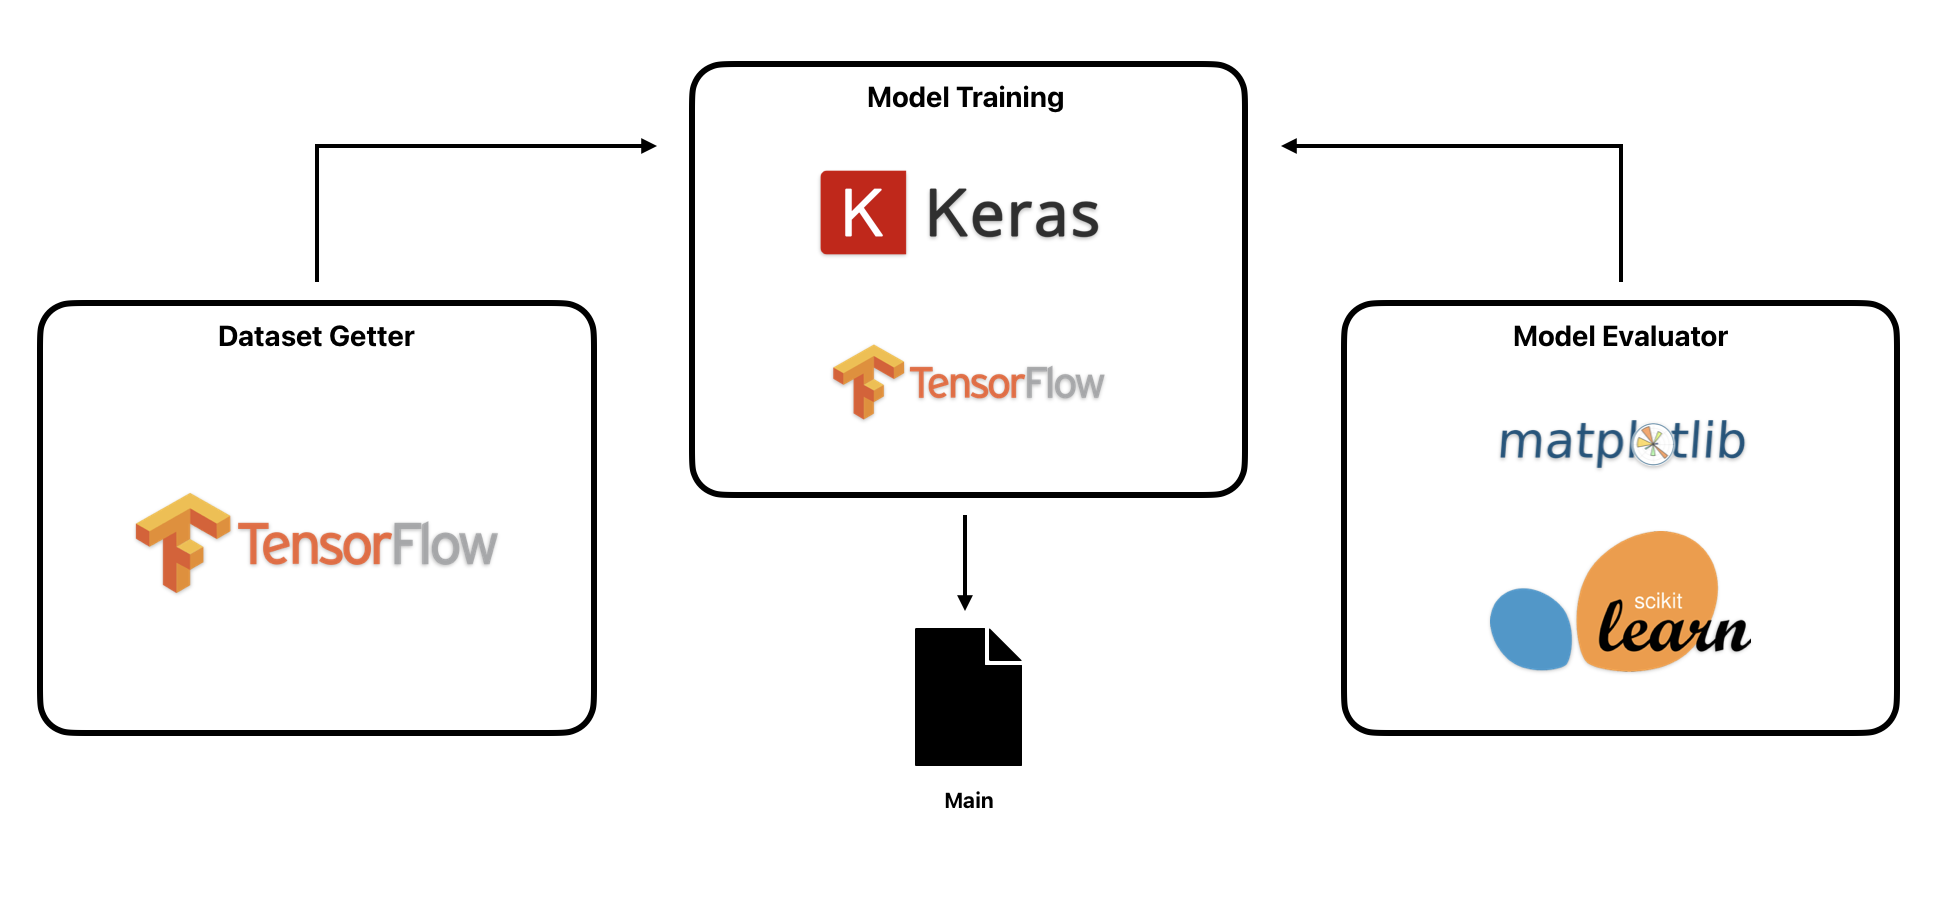
\includegraphics[alt={Architettura generale con le principali tecnologie utilizzate}, width=0.9\columnwidth]{img/design.png}
    \caption{\centering Architettura generale con le principali tecnologie utilizzate}
    \label{fig:desc-proj}
\end{figure}\noindent
L'applicazione progettata la si può vedere in tre macro sezioni, dove la principale di esse è quella che si occupa di effettuare l'addestramento delle reti neurali artificiali.\\
Per soddisfare i requisiti ho deciso di realizzare un semplice programma in Python utilizzabile dal terminale, quindi senza nessuna interfaccia grafica.
Questa scelta è dovuta sia dal fatto che non era richiesto per i requisiti, che dal fatto che non è necessario semplificare troppo l'utilizzo del programma, siccome ci si aspetta che l'utente finale sia già esperto e che voglia una certa libertà nella modifica dei parametri che vuole cambiare.\\
Ho deciso di progettare il programma incentrando tutto sul componente dedicato a svolgere gli addestramenti. Questo componente possiede due dipendenze, che sono: il componente dedicato all'ottenimento dei dati e il componente che si occupa di valutare il risultato.

\subsection{Addestramento di modelli}\noindent
Il \textit{focus} principale del programma è di creare modelli tramite l'addestramento di reti neurali artificiali. Per fare ciò ho utilizzato, come tecnologia principale, Keras.\\
Attraverso questa tecnologia è possibile creare modelli attraverso due API che sono disponibili all'utilizzo. Il loro funzionamento non è dissimile, ma possiedono delle caratteristiche fondamentali da capire:
\begin{itemize}
    \item \textbf{\textit{Sequential} API:} attraverso questa API la definizione dei modelli è veramente molto semplice, e risulta molto semplice anche il loro utilizzo. Però questa semplicità avviene ad un costo: ovvero che non è possibile inserire più \textit{input} di diverso tipo in contemporanea. Questo perchè i modelli che si possono definire, sono sequenziali e perciò sono una singola catena di processamento.
    \item \textbf{\textit{Functional} API:} attraverso questa API si possono definire modelli più complessi, ma anche l'utilizzo e definizione diventano relativamente più complessi. Questa intricatezza permette di creare modelli che supportano \textit{multi-input}, \textit{multi-output} oppure entrambi. 
\end{itemize}
\begin{figure}[H]
    \centering
    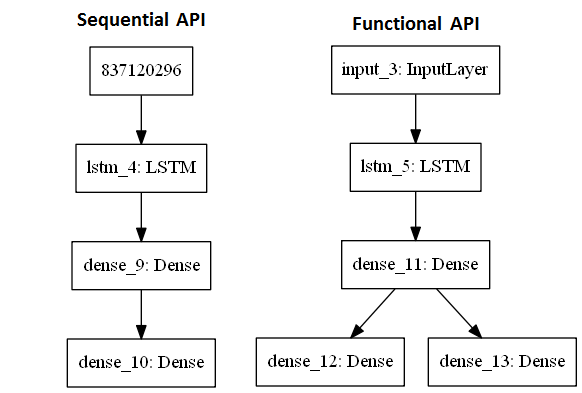
\includegraphics[alt={Confronto tra \textit{Sequential} API e \textit{Functional} API}, width=0.8\columnwidth]{img/seq-fun.png}
    \caption[Confronto tra \textit{Sequential} API e \textit{Functional} API]{\centering Confronto tra \textit{Sequential} API e \textit{Functional} API \par \textbf{Fonte:} \href{https://stackoverflow.com/questions/58092176/keras-sequential-vs-functional-api-for-multi-task-learning-neural-network}{stackoverflow.org}}
    \label{fig:desc-proj}
\end{figure}\noindent
Il programma da me progettato, include entrambe le API. L'utilizzo di una di esse viene deciso dall'utente nel \textit{file} principale di esecuzione del programma.\\
La scelta di implementare entrambe deriva dal fatto che l'utente finale necessita di confrontare l'influenza delle informazioni aggiuntive che vengono inserite nel modello sulle prestazioni finali ottenute. In questo specifico ambito, non è detto che informazioni aggiuntive come l'età e il peso del paziente influiscano notevolmente sulle prestazioni del modello creato.\\
Da un punto di vista teorico, le informazioni aggiuntive influiscono in modo positivo sulle prestazioni, però questa aggiunta espande il modello, e facendo ciò, vengono incrementati anche i requisiti prestazionali della macchina che deve eseguirlo.\\
Perciò ho deciso di implementare le due API sotto forma di due classi che implementano la stessa classe astratta, in modo da avere in comune più codice possibile.
\begin{figure}[H]
    \centering
    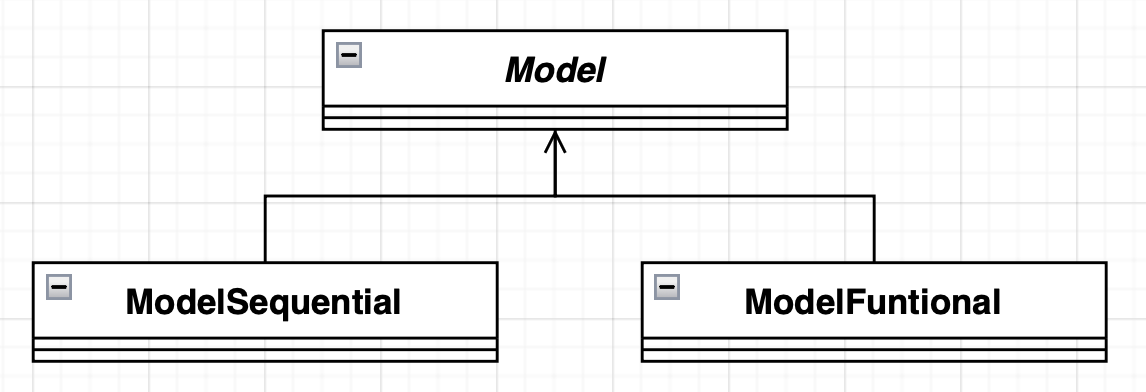
\includegraphics[alt={Diagramma delle classi di addestramento di reti neurali artificiali}, width=0.75\columnwidth]{img/model-diag.png}
    \caption{\centering Diagramma delle classi di addestramento di reti neurali artificiali}
    \label{fig:datasetgetter-diagram}
\end{figure}

\subsection{Gestione del \textit{dataset}}\noindent
Una delle dipendenze della parte di addestramento dei modelli è l'ottenimento dei dati su cui eseguire l'addestramento. Questo è un'importante passo negli addestramenti di reti neurali artificiali, senza di esso non sarebbe possibile neanche realizzare un singolo modello.\\
Per far sì che un addestramento avvenga, è necessario che i dati richiesti dall'addestramento stesso, siano disponibili all'interno della RAM, ma per fare ciò, ci sono due metodi:
\begin{itemize}
    \item \textbf{Caricare l'intero \textit{dataset}:} questa è l'opzione più semplice da realizzare. Ha il vantaggio di predisporre tutti i dati necessari in una memoria veloce come la RAM, permettendo tempi di risposta tra le varie \glslink{epoch}{epoche} veramente bassi. Tuttavia, questo metodo viene utilizzato solo quando il \textit{dataset} utilizzato non è tanto grande, siccome più grande un \textit{dataset} è, più RAM è richiesta.
    \item \textbf{Caricare in modo dinamico:} questa opzione risolve il problema del limite della RAM. I file richiesti durante l'addestramento vengono letti dalla memoria per l'archiviazione a lungo termine quando sono necessari, o se si utilizza il \gls{prefetch}, momenti prima. Perciò i dati permangono per poco tempo all'interno della RAM prima di essere rimpiazzati dai dati successivi. Questo permette di utilizzare \textit{dataset} di qualsiasi dimensione per addestrare reti neurali artificiali in qualsiasi macchina si voglia. Lo svantaggio di questa tecnica è che è subisce un \textit{bottleneck} nel caso si sta addestrando un modello computazionalmente semplice. Questo per via del limite fisico dovuto alla lettura dei dati dalla memoria di archiviazione a lungo termine.
\end{itemize}
Questo progetto, come spiegato precedentemente, tratta di \textit{dataset} di grandi dimensioni, perciò posso considerare di sviluppare solo la seconda delle due opzioni qui sopra presentate.\\
Per implementare ciò, ho scelto di utilizzare i \textit{generator} disponibili utilizzando TensorFlow, essendo completamente compatibile con l'addestramento effetuato con Keras. Ero però dubbioso in che formato era meglio mantenere il \textit{dataset} per ottenere i migliori risultati di velocità nel caricamento dei dati.\\
Per capire ciò, ho sperimentato utilizzando diversi formati di file per cercare di ottenere il miglior compromesso tra dinamicità e velocità.\\
Prima di esporre quale soluzione ho deciso di utilizzare alla fine, vado ad esporre una delle soluzioni che ho sperimentato.
Essa era stata ideata basandosi sulla riduzione dei tempi di caricamento dei vari file, riducendo il numero di file da caricare.
Per fare ciò ho compresso i \textit{file} originali del \textit{dataset}, in vari file HDF5, un formato di \textit{file} progettato per la memorizzazione di grandi quantità di dati, in modo da avere un numero minore di \textit{file} con una dimensione leggermente più grande.
Questo ha permesso di avere tempi di risposta minori tra una epoca e l'altra nella fase di addestramento.
Ma è anche vero che questa soluzione possedeva due problemi:
\begin{itemize}
    \item \textbf{Gestione delle \gls{label}:} questa soluzione complicava la gestione delle etichette associate ai dati, che erano ora in gruppi di \textit{file}. Una possibile soluzione avrebbe portato a progettare un sistema più complicato del necessario, e avrebbe portato via molto tempo.
    \item \textbf{Troppa specificità:} decidere quanti dati inserire in un HDF5 \textit{file} è di per sè un dilemma. La dimensione di certi \textit{file} potrebbe andare bene per un \textit{computer}, ma non è detto che sia la scelta più ottimale per'altro. Inoltre il vantaggio viene perso se si svolge addestramenti di modelli computazionalmente demandanti.
\end{itemize}
Perciò, considerando tutte le opzioni, ho deciso che era meglio mantenere i vari dati del \textit{dataset} nel loro formato originale. Per il semplice fatto che questa soluzione avrebbe portato alla minore produzione di codice, che è importante da considerare, siccome richiede meno modifiche in futuro, nel caso ce ne fosse bisogno.\\
Ho progettato questo componente similmente al componente precedentemente esposto: ovvero tramite una classe astratta da dove vengono implementate diverse classi concrete.
In questo caso, avere la classe astratta è di maggiore importanza. Questo perchè oltre a creare le due classi per dare l'\textit{input} alle due API, che ne richiedono due diversi, dovevo implementare anche un generatore per i \textit{file} \gls{dicom} che facevano parte del piccolo \textit{dataset} privato.
Questi \textit{file} sono una piccolissima frazione del \textit{dataset} con cui l'azienda si troverà a lavorare in futuro, perciò come da requisiti, dovevo implementarli per validare la possibilità di utilizzarli nel codice da me prodotto.
\begin{figure}[H]
    \centering
    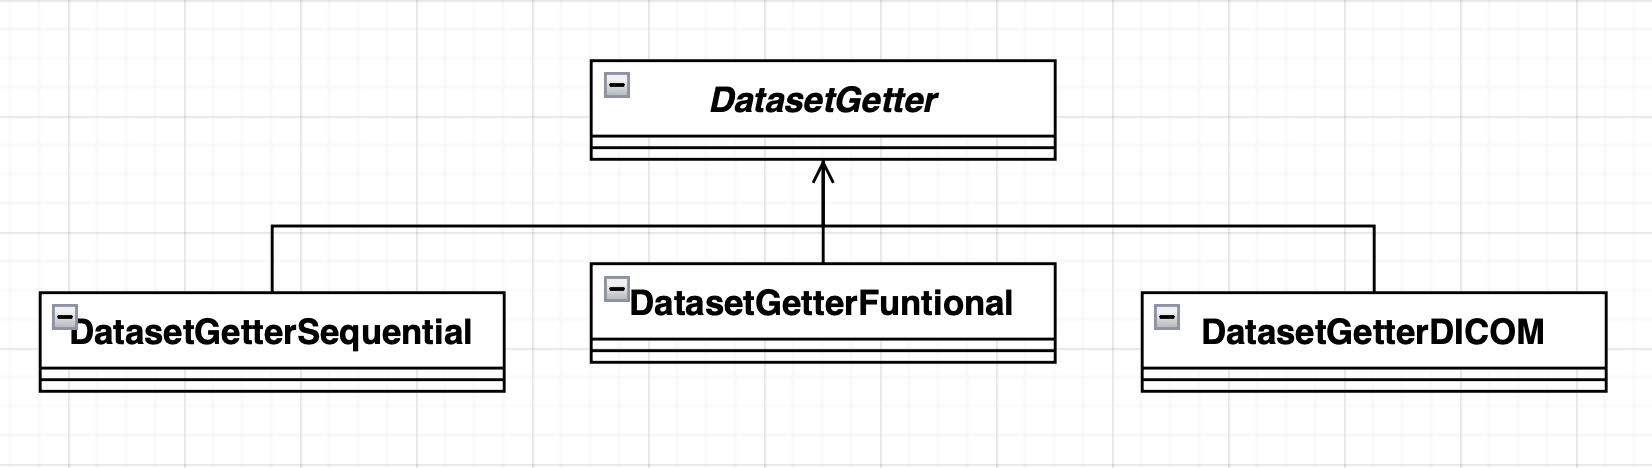
\includegraphics[alt={Diagramma delle classi di gestione del \textit{dataset}}, width=0.9\columnwidth]{img/dg-diag.png}
    \caption{\centering Diagramma delle classi di gestione del \textit{dataset}}
    \label{fig:datasetgetter-diagram}
\end{figure}

\subsection{Valutazione dei modelli}\noindent
L'ultima dipendenza per l'addestramento delle reti neurali artificiali è la realizzazione di vari \textit{output} che danno la possibilità di valutare oggettivamente le prestazioni del modello creato.\\
A fine dell'addestramento, il componente a esso dedicato si occupa di chiamare questo componente, che ricevendo determinate informazioni dell'addestramento, si occupa di generare le varie metriche richieste dai requisiti.
\newpage\noindent
Di seguito vado ad esporre le metriche implementate:
\begin{itemize}
    \item \textbf{Grafici di andamento del \textit{training}:} durante l'addestramento, Keras, si occupa di valutare l'andamento. Prendendo le informazioni collezionate da Keras, è possibile creare dei grafici, utili per valutare varie cose.
    \item \textbf{\glslink{confusionmatrix}{Matrice di confusione}:} ``strumento'' utilizzato per comparare le predizioni di \textit{test} che un modello svolge, con gli effettivi risultati.
    \item \textbf{\glslink{confidence}{Confidenza}:} generalmente un'istogramma dove viene visualizzata l'incertezza del modello nelle predizioni che svolge durante la fase di \textit{test}.
    \item \textbf{Varie statistiche:} si tratta di una lista di metriche in forma testuale, che valuta numericamente le prestazioni del modello nel predirre. Una delle metriche più notevoli è quella dell'accuratezza, che indica la proporzione di predizioni corrette rispetto al numero totale di predizioni effettuate.
\end{itemize}
Per la realizzazione dei grafici ho deciso di utilizzare la libreria Matplotlib, mentre per la matrice di confusione e le varie statistiche, ho scelto di usare la libreria: Scikit-learn.\\
Inoltre, questo componente si occupa di salvare i modelli che sono stati creati durante l'apprendimento in una specifica \textit{directory}, insieme a tutte le metriche qui sopra esposte.

\section{Codifica}\label{sec:coding}\noindent
% \texttt{Descrizione dell'attività di codifica.}
In questa sezione vado a descrivere come ho svolto la fase di codifica del progetto, mi soffermerò a descrivere alcune parti di codice che ritengo notevoli di attenzione.

\subsection{Prototipo}\noindent
Prima ancora di iniziare a realizzare quello che verrà considerato il prodotto finale, ho creato un prototipo che mi ha aiutato nella fase di progettazione.\\
Questo prototipo ha racchiuso, semplificando, i vari punti del progetto in un singolo \textit{file} eseguibile, che quindi possedeva tutta la \textit{pipeline} di: gestione del \textit{dataset}, addestramento delle reti neurali artificiali e la valutazione del modello creato.\\
Grazie ad esso ho potuto sperimentare vari modi per caricare il \textit{dataset} in RAM per effettuare l'addestramento in modo efficiente.\\
Di seguito vado a esporre la versione finale che ho ottenuto dopo la fase di sperimentazione:
\begin{listing}[H]
    \inputminted{python}{code/generator.py}
    \caption{Codice della variabile del generatore}
    \label{listing:py_gen_var}
\end{listing}\noindent
Il \textit{dataset} viene visto all'interno del programma come una variable, questa è un \texttt{tf.data.Dataset} della libreria TensorFlow, che è un \textit{input} supportato da Keras per la creazione di un modello.
Da notare nel codice \ref{listing:py_gen_var} è che in ultima riga viene applicato il \textit{prefetch}, che in questo caso si occupa di ottenere, oltre al dato necessario al momento, anche i prossimi due dati richiesti. Questi dati sono stati raggruppati in \gls{batch}, perciò non viene preso un singolo dato per processare, ma un piccolo gruppo.\\
La definizione del generatore avviene tramite la funzione visibile in \ref{listing:py_gen_fun}.
Essa si occupa di prelevare le informazioni che sono contenute in uno specifico file, che contiene i percorsi \textit{file} dei vari dati, oltre che a informazioni aggiuntive associate a quest'ultimi, come le \textit{label}.
Successivamente si occupa di dichiarare il generatore dei dati, applicando una determinata struttura, e ritorna la variabile.
\begin{listing}[H]
    \inputminted{python}{code/generator_fun.py}
    \caption{Codice della funzione che definisce il generatore}
    \label{listing:py_gen_fun}
\end{listing}\noindent
La funzione che effettivamente ``genera'' i dati, raffigurata in \ref{listing:py_gen_base}.
\begin{listing}[H]
    \inputminted{python}{code/generator_base.py}
    \caption{Parte di codice che sfrutta il commando \texttt{yield}}
    \label{listing:py_gen_base}
\end{listing}\noindent
Questa funzione prende ogni singolo elemento della lista e ritorna una sorta di iteratore tramite il commando \texttt{yield} di Python.
Gli elementi che vengono restituiti sono il segnale elettrocardiografico e la \textit{label} ad esso associato, che a loro volta sono stati ricavati con le seguenti funzioni:
\begin{listing}[H]
    \inputminted{python}{code/generator_final.py}
    \caption{Codice delle funzioni che ottengono gli effettivi dati}
    \label{listing:py_gen_final}
\end{listing}\noindent
Nel codice \ref{listing:py_gen_final}, possiamo vedere come vengono gestiti gli elettrocardiogrammi e le \textit{label.}\\
Nel caso degli elettrocardiogrammi, in questo esempio stavo utilizzando il \textit{dataset} pubblico PTB-XL, che salva ogni singolo segnale all'interno di un WFDB (\textit{WaveForm DataBase}), ovvero una struttura specifica per memorizzare segnali di dati fisiologici. Essi vengono letti attraverso la funzione: \texttt{wfdb.rdsamp()}.\\
Per quanto riguarda le \textit{label}, esse originano dalla lista che viene letta all'interno di \ref{listing:py_gen_fun}. Nella lista sono segnate in varie superclassi, ma in questo esempio vengono trasformate in valore binario: `0' nel caso di pazienti sani, `1' nel caso di pazienti con patologie.

\subsection{Gestione del \textit{dataset}}\noindent
Quando sono passato a realizzare questo componente nel prodotto finale, il codice che ho utilizzato non differenzia moltissimo da quello che ho appena spiegato qui sopra.
Però dovevo accomodare il supporto ad altre ``versioni'' del \textit{dataset}. Di seguito illustro due di queste versioni.\\
La prima versione che voglio esporre è quella che oltre al segnale elettrocardiografico, include anche altre informazioni del paziente:
\begin{listing}[H]
    \inputminted{python}{code/generator_additional.py}
    \caption{Codice del generatore di dati che include informazioni aggiuntive}
    \label{listing:py_gen_additional}
\end{listing}\noindent
Con il codice \ref{listing:py_gen_additional} voglio notare che la maggior parte delle modifiche che vengono svolte sono nelle funzioni che utilizzano il \texttt{yield} di Python e la funzione che si occupa di ricavare gli effettivi dati.\\
La versione di codice che ho incluso qua fa parte della versione finale (in parte tagliata per questioni di spazio), ed è per questo che nella funzione \texttt{\textunderscore load\textunderscore single\textunderscore ecg()} sono presenti anche i richiami per le funzioni di \textit{downsampling} e di \textit{preprocessing}, due procedimenti che erano richiesti dai requisiti.\\
La seconda versione che volevo mostrare era l'implementazione del supporto per i \textit{file} DICOM:
\begin{listing}[H]
    \inputminted{python}{code/generator_dicom.py}
    \caption{Codice del generatore di dati attraverso \textit{file} DICOM}
    \label{listing:py_gen_dicom}
\end{listing}\noindent
Anche nel codice \ref{listing:py_gen_dicom} è possibile notare che la maggior parte del codice rimane la stessa, con differenza di come viene letto il \textit{file}. Essendo un formato diverso, il \textit{file} DICOM non viene più letto attraverso \texttt{wfdb.rdsamp()}, ma attraverso \texttt{dcmread()}.

\subsection{Addestramento di reti neurali artificiali}\noindent
La componente per l'addestramento di reti neurali artificiali sarà la parte unisce le altre componenti per realizzare gli obiettivi del progetto, però è anche quella che è possiede meno codice rispetto alle altre componenti.
Questo è dovuto principalmente dalla semplicità di utilizzo delle API di Keras. A riguardo di questo, voglio mostrare la differenza delle due API utilizzabili, che ho mezionato nella sezione di progettazione.\\
Inizio illustrando con un'esempio di modello che utilizza la \textit{Sequential} API:
\begin{listing}[H]
    \inputminted{python}{code/model_sequential.py}
    \caption{Esempio di definizione di un modello con la \textit{Sequential} API}
    \label{listing:py_model_seq}
\end{listing}\noindent
In \ref{listing:py_model_seq} possiamo notare che la definizione è racchiusa in una singola variabile. I modelli sono realizzati a strati, dove ogni strato realizza ognuno una specifica operazione.
L'\textit{input} viene processato uno strato alla volta, dall'alto verso il basso, dove viene restituito l'\textit{output}.\\
\begin{listing}[H]
    \inputminted{python}{code/model_functional.py}
    \caption{Esempio di definizione di un modello con la \textit{Functional} API}
    \label{listing:py_model_fun}
\end{listing}\noindent
Mentre osservando l'esempio di \textit{Functional} API, rappresentato nel codice \ref{listing:py_model_fun}, possiamo vedere che vengono dichiarate diverse variabili prima di dichiarare l'effettiva struttura finale del modello.
Questo perchè vengono creati diverse strutture sequenziali che vengono unite alla fine per creare un singolo modello.\\
Nell'ultimo esempio mostrato, ho creato due ``\textit{pipeline}'' per processare i segnali elettrocardiografici e le infomazioni aggiuntive dei pazienti, rispettivamente tramite \texttt{x1} e \texttt{x2}.
Questi due elementi sequenziali uniscono il loro ultimo strato in un nuovo elemento sequenziale, \texttt{x}, che si occuperà di restituire l'\textit{output} finale del modello.

\subsection{Menzioni onorevoli}\noindent
Per finire, vado a parlare di alcune altre parti di codice, non troppo rilevanti ma che meritano almeno una piccola menzione.\\
Una di esse è la componente che viene utilizzata quando il l'addestramento viene terminato, ovvero la componente di valutazione del modello creato.
Ho codificato una semplice classe che raccoglie tutte le funzioni che generano le metriche necessarie per la valutazione, come ad esempio \ref{listing:py_eval}.
\begin{listing}[H]
    \inputminted{python}{code/evaluation_example.py}
    \caption{Esempio di funzione per la valutazione dei modelli}
    \label{listing:py_eval}
\end{listing}\noindent
Inoltre, questa componente utilizza varie funzioni che ho creato per il salvataggio delle metriche e modelli create durante esecuzione del programma.\\
Infine, per facilitare la modifica di variabili che si trovano in diverse parti del codice, ho creato una classe che si occupa di restituire i valori configurati in \texttt{config.json} dove è necessario, semplificando l'utilizzo del programma all'utente.

\section{Verifica e validazione}\label{sec:test-validation}\noindent
% \texttt{Descrizione delle attività di verifica e validazione.}
Per questo processo di sviluppo del software ho svolto principalmente due cose.
La prima è stata di realizzare alcuni \textit{unit test}, soprattutto per controllare il corretto funzionamento delle funzioni che si occupano di gestire la trasformazione delle \textit{label}.
Fare ciò è abbastanza importante, questo perchè se le \textit{label} vengono trasformate in un modo da non essere più veritiere quando vengono associate al proprio dato, allora quando esse vengono utilizzate per l'addestramento, il modello che ne risulterà fuori sarà inutilizzabile nel mondo reale.\\
Mentre per il resto ho adottato un approccio manuale, controllando personalmente le varie parti del programma.
Questo per via dell'ambito in cui il progetto si occupava, ovvero quello del \textit{machine learning}. In questo campo la realizzazione dei vari \textit{test} risulta parecchio complicata, dovuto principalmente dalla natura probabilistica e dinamica dei modelli di predizione.\\
Per questo, mi è risultato più semplice e veloce nel controllare personalmente se le modifiche che svolgevo causavano problemi o meno.

\section{Risultati raggiunti}\label{sec:results}

\subsection{Piano qualitativo}\noindent
% \texttt{Esposizione dei risultati ottenuti sul piano qualitativo, dove viene visto il prodotto in una visione d'insieme.}
Il prodotto che ho realizzato lo si può definire come uno strumento utilizzabile per la creazione di modelli tramite l'addestramento di reti neurali artificiali.\\
In esso, l'utente può definire la struttura di modello su cui vuole svolgere l'addestramento, può definire se vuole o meno applicare funzionalità come il \textit{downsampling} oppure il \textit{preprocessing} e infine può valutare le prestazioni di quello che ha ottenuto.\\
Questo strumento supporta diverse modalità di \textit{training}, inoltre, il cambiamento da una modalità è agevolato da un \textit{file} di \textit{config}, dove si possono modificare anche altre impostazioni. Raffiguro questo \textit{file} attraverso \ref{fig:config}.
\begin{figure}[H]
    \centering
    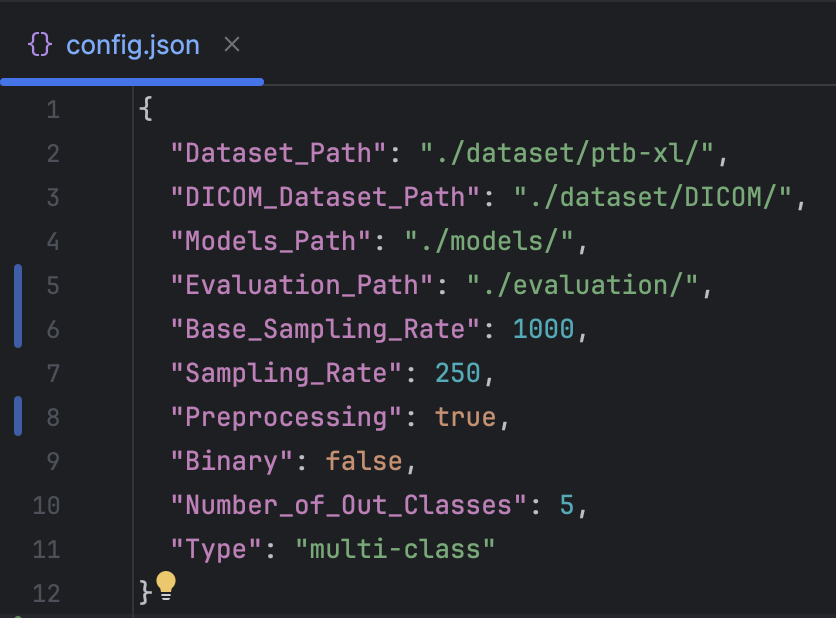
\includegraphics[alt={Cattura dello schermo rappresentante il \textit{file} di \textit{config}}, width=0.8\columnwidth]{img/config.png}
    \caption{\centering Cattura dello schermo rappresentante il \textit{file} di \textit{config}}
    \label{fig:config}
\end{figure}\noindent
A fine dell'esecuzione del programma, l'utente può trovare le varie valutazioni all'interno di una cartella specifica contenuta nella \textit{directory} del progetto. Di seguito mostro un'esempio dei contenuti prodotti:
\begin{figure}[H]
    \centering
    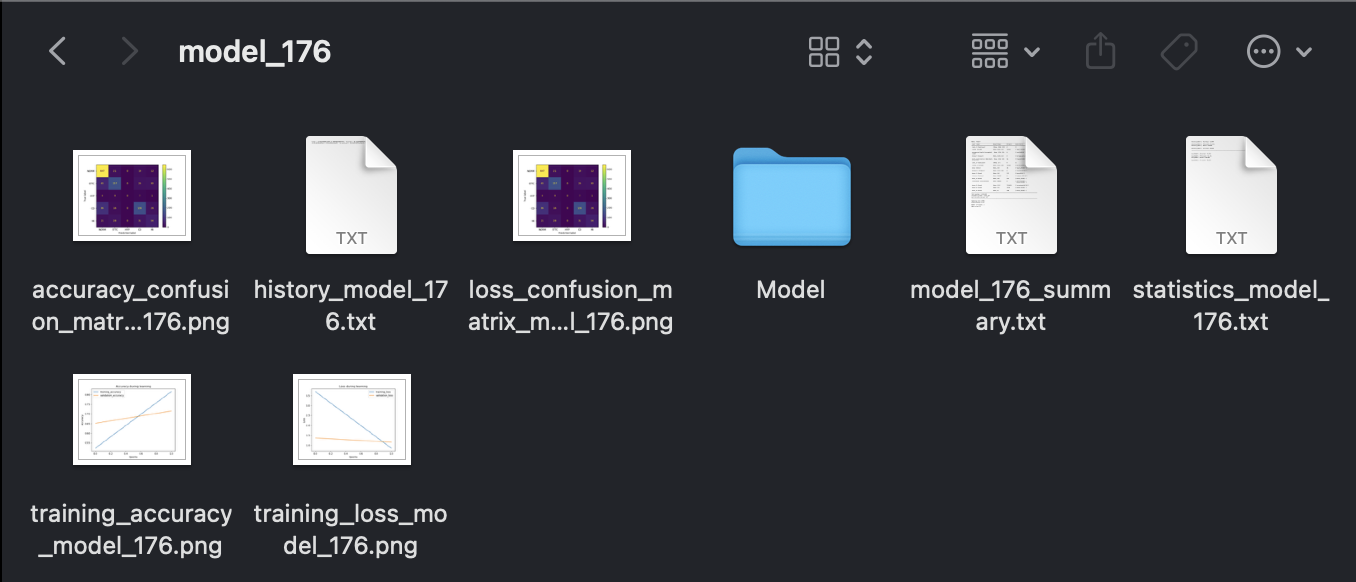
\includegraphics[alt={Cattura dello schermo rappresentante i \textit{file} di \textit{output}}, width=0.9\columnwidth]{img/output.png}
    \caption{\centering Cattura dello schermo rappresentante i \textit{file} di \textit{output}}
    \label{fig:output}
\end{figure}\noindent
Inoltre, durante allo \textit{stage} avevo l'obiettivo di realizzare io stesso dei \textit{training} di reti neurali artificiali.
Perciò ho anche prodotto due modelli cercando di ottenere delle buone prestazioni. Essi sono due perchè ho salvato solo i risultati migliori che ho ottenuto per due tipi di classificazione: binaria, ovvero sano o non sano, e multi-classe, dove il modello predice il risultato su cinque possibili classi.

\subsection{Piano quantitativo}\noindent
% \texttt{Esposizione dei risultati ottenuti sul piano quantitativo, qui vengono illustrate la copertura dei requisiti e dei test.}
Sul piano quantitativo sono riuscito a soddisfare tutti i requisiti derivanti dall'analisi dei requisiti e rappresentati nella tabella \ref{tab:user-stories}.\\
Per quanto riguarda il \textit{code coverage}, non avendo creato solo test automatici, ma svolto test manuali per via della natura del progetto: non posso quantificare in modo obiettivo questa metrica.\\
Tuttavia posso parlare dei risultati ottenuti con l'attività di addestramento.
\begin{center}
    \rowcolors{1}{}{tableGray}
    \begin{longtable}{|p{2.5cm}|p{2.5cm}|}
    \hline
    \multicolumn{2}{|c|}{\textbf{\textit{Binary model}}} \\ 
    \hline 
    \endfirsthead
    \rowcolor{white}
    \multicolumn{2}{c}{{\bfseries \tablename\ \thetable{} -- Continuo della tabella}}\\
    \hline
    \multicolumn{1}{|c|}{\textbf{Identificatore}} & \multicolumn{1}{c|}{\textbf{\textit{User story}}}\\ \hline 
    \endhead
    \hline
    \rowcolor{white}
    \multicolumn{2}{|r|}{{Continua nella prossima pagina...}}\\
    \hline
    \endfoot
    \endlastfoot
    
    \multicolumn{1}{|c|}{\textit{Accuracy}} & \multicolumn{1}{|c|}{86.25\%} \\
    \hline
    \multicolumn{1}{|c|}{\textit{Precision}} & \multicolumn{1}{|c|}{87.93\%} \\
    \hline
    \multicolumn{1}{|c|}{\textit{Recall}} & \multicolumn{1}{|c|}{81.07\%} \\
    \hline
    \multicolumn{1}{|c|}{\textit{Specificity}} & \multicolumn{1}{|c|}{90.63\%} \\
    \hline
    \multicolumn{1}{|c|}{\textit{F1 Score}} & \multicolumn{1}{|c|}{84.36\%} \\
    \hline
    \hiderowcolors
    \caption{Tabella contenente le prestazioni del modello binario.}
    \label{tab:bin-model-res}
    \end{longtable}

    \rowcolors{1}{}{tableGray}
    \begin{longtable}{|p{2.5cm}|p{2.5cm}|}
    \hline
    \multicolumn{2}{|c|}{\textbf{\textit{Multi-class model}}} \\ 
    \hline 
    \endfirsthead
    \rowcolor{white}
    \multicolumn{2}{c}{{\bfseries \tablename\ \thetable{} -- Continuo della tabella}}\\
    \hline
    \multicolumn{1}{|c|}{\textbf{Identificatore}} & \multicolumn{1}{c|}{\textbf{\textit{User story}}}\\ \hline 
    \endhead
    \hline
    \rowcolor{white}
    \multicolumn{2}{|r|}{{Continua nella prossima pagina...}}\\
    \hline
    \endfoot
    \endlastfoot
    
    \multicolumn{1}{|c|}{\textit{Accuracy}} & \multicolumn{1}{|c|}{71.50\%} \\
    \hline
    \multicolumn{1}{|c|}{\textit{Precision}} & \multicolumn{1}{|c|}{51.11\%} \\
    \hline
    \multicolumn{1}{|c|}{\textit{Recall}} & \multicolumn{1}{|c|}{48.85\%} \\
    \hline
    \multicolumn{1}{|c|}{\textit{F1 Score}} & \multicolumn{1}{|c|}{49.65\%} \\
    \hline
    \hiderowcolors
    \caption{Tabella contenente le prestazioni del modello multi-classe.}
    \label{tab:multiclass-model-res}
    \end{longtable}
\end{center}\noindent
Come si può vedere nelle tabelle \ref{tab:bin-model-res} e \ref{tab:multiclass-model-res}, i modelli creati da me non sono veramente ottimi, sopratutto se vengono seguiti gli \textit{standard} richiesti in campo medico, dove si richiede un'accuratezza più alta possibile.\\
Tuttavia, questi risultati non sono troppo dovuti a delle mie scarse configurazioni, ma al \textit{dataset} utilizzato.
Avendo utilizzato per la maggior parte il \textit{dataset} pubblico PTB-XL di PhysioNet, ho potuto confrontare i miei risultati ottenuti con una ricerca scientifica che ha svolto i miei stessi tipi di addestramenti di reti neurali artificiali.\\
Il \textit{paper} scientifico in questione è \citetitle{article:ecg-paper}, dove vengono mostrati dei risultati finali simili a quello che ho ottenuto, solo marginalmente migliori.
    \chapter{Retrospettiva}
\label{chap:retrospettiva}

\section{Conseguimento degli obiettivi}

\subsection{Obiettivi aziendali}\noindent
Esposizione degli obiettivi aziendali raggiunti, facendo riferimento agli obiettivi descritti nelle sezioni precedenti.

\subsection{Obiettivi personali}\noindent
Esposizione degli obiettivi personali raggiunti, facendo riferimento agli obiettivi descritti nelle sezioni precedenti.

\section{Competenze acquisite}\noindent
Descrizione della maturazione professionale, in ambito di conoscenze e abilità.

\section{Divario tra università e lavoro}\noindent
Descrizione della distanza tra le competenze imparate in università e quelle richieste allo \textit{stage}.

    \pagenumbering{roman}
    \backmatter
    \chapter{Bibliografia}
\label{cap:bibliography}

\nocite{*}

% Books bibliography
\printbibliography[heading=subbibliography, title={Testi}, type=book]

% Articles bibliography
\printbibliography[heading=subbibliography, title={Articoli}, type=article]

% Websites bibliography
%\printbibliography[heading=subbibliography, title={Siti}, type=online]

    \chapter{Sitografia}
\label{cap:webliography}
\nocite{*}

% Websites bibliography
\printbibliography[heading=subbibliography, title={\null}, type=online]

\end{document}